
\chapter{Make - Understanding the Molecular Transformer}\label{ch:transformer}
% \label{chap:MolTrans}

\begin{quote}
    This chapter is based on Dávid Péter Kovács, William McCorkindale and Alpha A. Lee. Quantitative interpretation explains machine learning models for chemical reaction prediction and uncovers bias. \textit{Nature Communications} volume 12, Article number: 1695 (2021)
\end{quote}

\noindent\hfil\rule{0.5\textwidth}{.4pt}\hfil


% \begin{abstract}
% Organic synthesis remains a a major challenge in drug discovery. Although a plethora of machine learning models have been proposed as solutions in the literature, they suffer from being opaque black-boxes. It is neither clear if the models are making correct predictions because they inferred the salient chemistry, nor is it clear which training data they are relying on to reach a prediction. This opaqueness hinders both model developers and users. In this paper, we quantitatively interpret the Molecular Transformer, the state-of-the-art model for reaction prediction. We develop a framework to attribute predicted reaction outcomes both to specific parts of reactants, and to reactions in the training set. Furthermore, we demonstrate how to retrieve evidence for predicted reaction outcomes, and understand counterintuitive predictions by scrutinising the data. Additionally, we identify Clever Hans predictions where the correct prediction is reached for the wrong reason due to dataset bias. We present a new debiased dataset that provides a more realistic assessment of model performance, which we propose as the new standard benchmark for comparing reaction prediction models.
% \end{abstract}

% \section*{\label{sec:intro}Introduction}

% Organic synthesis remains a challenge in small molecule drug design, sinking time in the design-make-test cycle and potentially limiting the complexity of chemical space being explored \cite{blakemore2018organic,bostrom2018expanding}. The challenge of synthesis planning lies in searching through myriad of possible reactions to find optimal routes, and in predicting whether each possible reaction is indeed feasible and high yielding for the particular substrate in question. The problem of efficient search in synthesis has been recently addressed, inspired by innovations in computer science on searching and gameplay \cite{segler2017neural,segler2018planning,kishimoto2019depth,schreck2019learning, segler2019world}. However, accurately predicting the outcome of chemical reactions remains a hurdle \cite{Coley2018, Johansson2020, Struble2020}.

% The current state-of-the-art in reaction prediction is the Molecular Transformer \cite{Schwaller2019}, which employs the transformer neural network architecture that was first introduced for neural machine translation \cite{Vaswani2017}. The input to the model is a text representation of the chemical structures of the reactant and reagent, and the model performs machine translation to predict most likely output molecule with a probability score. The Molecular Transformer achieves a 90\% Top-1 accuracy on the USPTO dataset of organic reactions that was text mined from US patents \cite{Lowe2012} and filtered \cite{Jin2017}. Recent work shows that thorough dataset augmentation improves model performance by allowing it to consider different equivalent SMILES representations \cite{tetko2020state}.

% However, a key stumbling block in the Molecular Transformer is the lack of interpretability. Why the Molecular Transformer predicts one reaction outcome over another, and which training set reactions it finds most similar when reaching a particular prediction, are both unclear. Quantitative interpretability is crucial to both model users and model developers. 

% For model users, interpretability is important because chemical reactions are highly contextual, with important anthropomorphic metadata that the model overlooks. For example, reactants, reagents and products are only a part of the reaction. The reaction conditions, the scale of a particular reaction (e.g. discovery chemistry or scale up), and scientific focus of the project (e.g. total synthesis, medicinal chemistry or methods development) are some of the context that a skilled chemist can employ to interpret and understand the reaction. 

% For model developers, physical organic chemistry principles explain chemical reactivity and selectivity. As such, probing whether rationales outputted by the Molecular Transformer are congruent with physics allows developers to interrogate whether the Molecular Transformer is getting the correct prediction for the right reasons, and design model improvements based on those insights. 

% In this paper, we develop a suite of methods that quantitatively interprets the Molecular Transformer by attributing predictions to the input chemical structure and the training data. We illustrate our two-prong approach via a series of sentinel examples,  showing how we uncovered what the model is learning, what it finds difficult, and explains its failure modes. Our method discovers hidden biases in the training data that hinder generalization performance and masks model shortcomings, which we resolved by introducing a new unbiased train / test split. 

% \begin{figure*}[ht!]
% 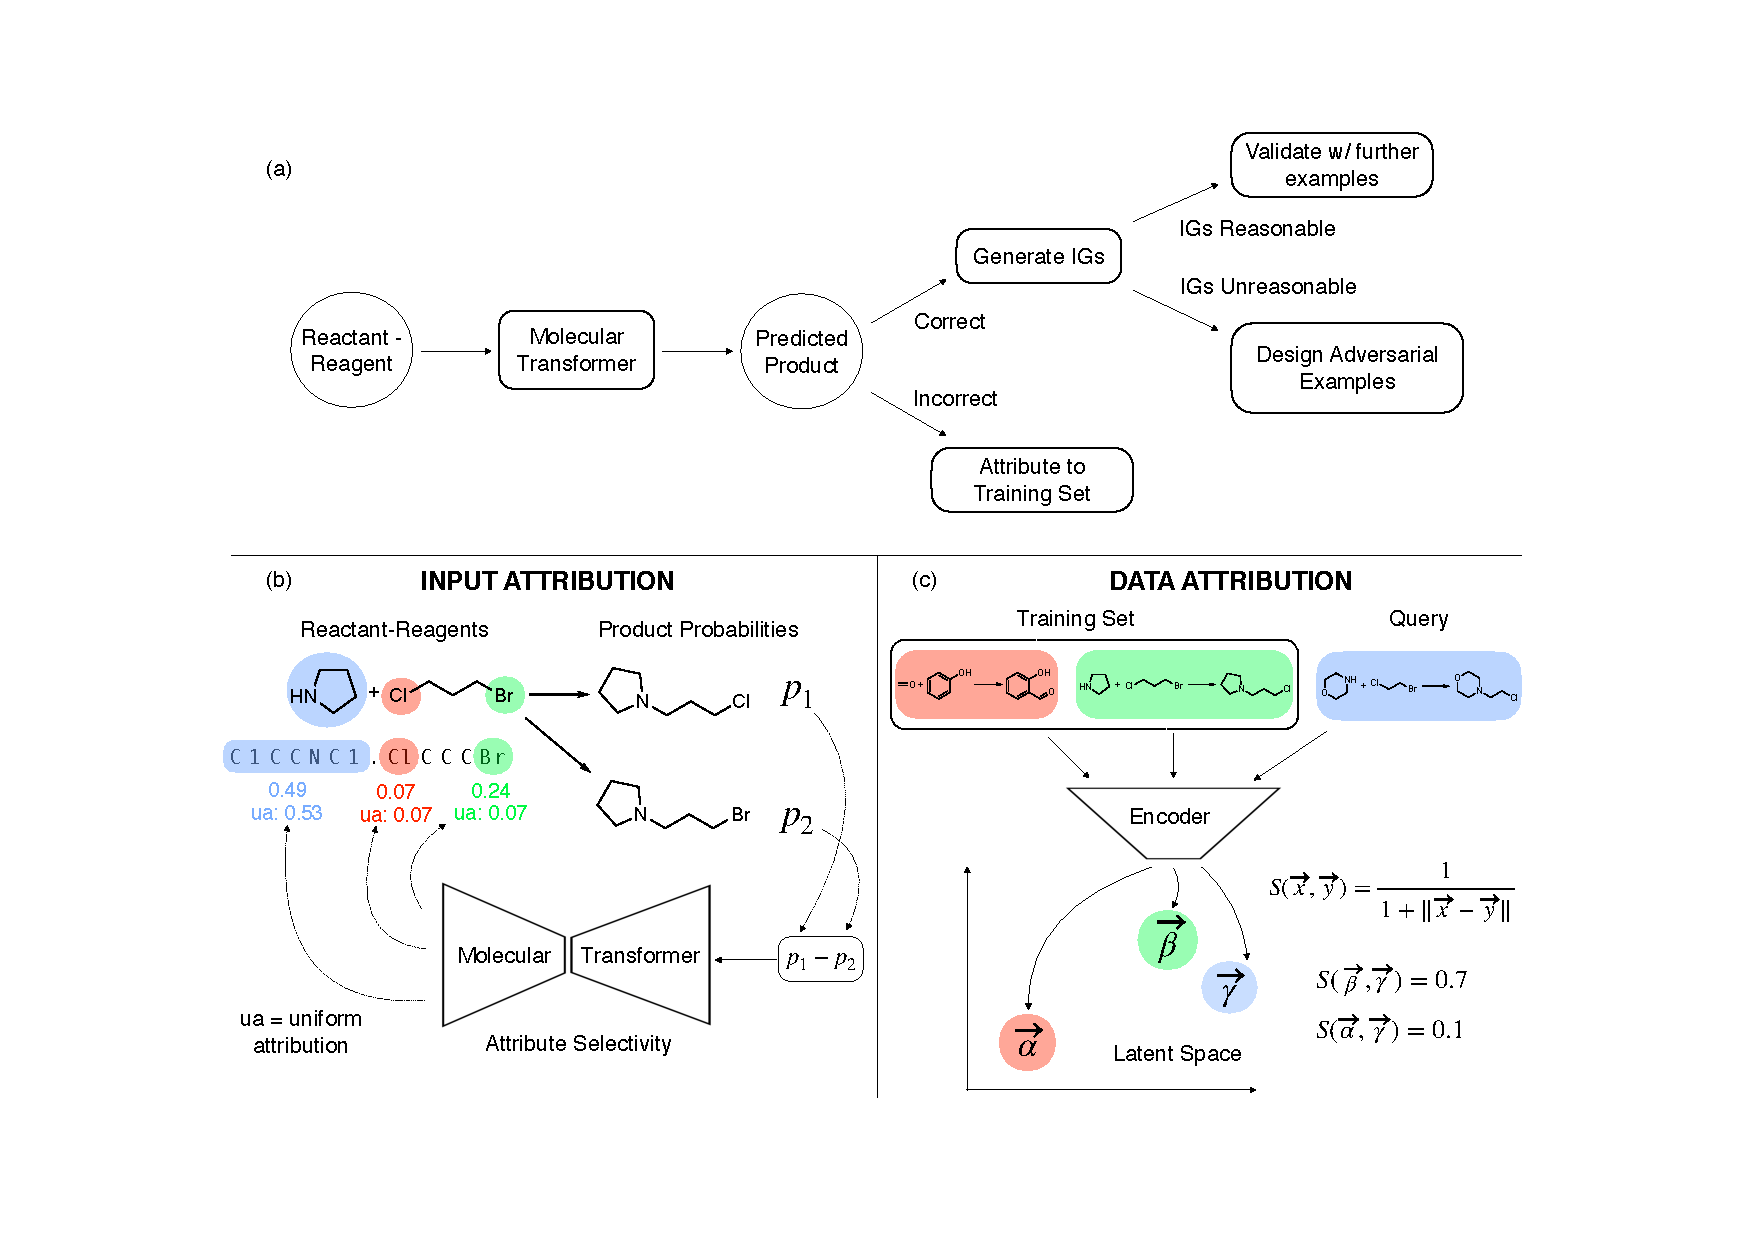
\includegraphics[width=0.8\textwidth]{Chapters/Transformer/Figs/workflow.pdf}
% \caption{\label{fig:workflow} \textbf{Schematic illustration of the attribution workflow} (a) Overview of our workflow to interpret the Molecular Transformer. (b) Schematic of how the predicted probability difference between two products are attributed back to the reactant-reagent string in order to interpret the model's understanding of selectivity. The IG attributions below the reactant SMILES are compared to the uniformly distributed probability difference (ua) below. (c) Schematic of how the latent space encoding of reactant-reagent strings are used to infer the learnt similarity between query reactants and those from the training set.}
% \end{figure*}

% \section*{Results}\label{sec:resu}
% \subsection*{Quantitative Interpretation}
% There are three key factors determining the prediction of a machine learning model: the architecture, the training data and the input. Neural network models are often considered as black-boxes because of the complex ways these three factors interact to yield a prediction. 

% To interpret model prediction, we first need to define what interpretability means. We suggest interpretability is the ability to discover associations and counterfactuals between input and output, and the ability to query evidence in the data supporting a certain outcome. Our approach follows the accepted scientific process: A scientific theory usually identifies factors that are related to a certain outcome and conversely how the absence of those factors is related to absence of outcome. Furthermore the investigator needs to show pieces of evidence that support the theory.

% We employ Integrated Gradients~\cite{Sundararajan2017} as a rigorous method for attributing the predicted probability difference of two plausible products of a selective chemical reaction to parts of the input. The attributions show how much each substructure is contributing to the predicted selectivity of the model. This is illustrated on Figure~\ref{fig:workflow}(b). The values of the attributions are compared to the value each subgroup would receive if the probability difference would be distributed evenly across the input. The parts of the structures getting higher IGs than the uniform attribution (ua) are considered important. For further description of our adaptation of IGs see Section~\ref{sec:methods}.\par

% Attributing the predictions of neural networks to most similar training data points is less widely researched. To achieve this goal we developed a new method based on the latent space similarity of the reactions. We used the outputs of the Molecular Transformer encoder averaged over the tokens to achieve a fixed length vector representation of the reactions. The most similar training reactions according the model were than identified using the Euclidean distance of these latent space vectors. A schematic overview of our method is shown on Figure~\ref{fig:workflow}(c). Details of the methods can be found in Section~\ref{sec:methods}. 

% We validate our interpretations in two ways. The first is via falsification. If the integrated gradients attributions are chemically unreasonable, i.e. predictions are correct for the wrong reasons, we design adversarial examples that force the model into wrong predictions. The second is by identifying causes for the prediction in the training data. If a prediction is wrong, we interrogate whether a similarly incorrect entry is in the training data. 

% \subsection*{Investigation of Specific Reaction Classes}

% We investigate in detail three reaction classes that are commonly used in medicinal chemistry. Through these examples we illustrate each of the three branches in Figure~\ref{fig:workflow}(a). We first examine the selective epoxidation of alkenes which is an example where the Molecular Transformer is producing the right prediction for the right reason. We then turn to the Diels-Alder reaction, which is a scaffold-building transformation widely used in synthesis. We show that the Molecular Transformer is not able to predict this reaction. Following the bottom branch of Figure~\ref{fig:workflow}(a) we investigate it using Data attribution and find that the USPTO dataset contains very few instances of Diels-Alder reactions, likely explaining why the model is not able to predict the outcome correctly.

%     Finally we consider the Friedel-Crafts acylation reactions of substituted benzenes. We show that the Molecular Transformer predicts the right product for the wrong reason and validate our interpretation using a number of adversarial examples. We also demonstrate with the help of an artificial dataset how this behaviour is the result of dataset bias. 
    
%     In light of the identified pathologies, we re-examine the reported 90\% accuracy of the Molecular Transformer and demonstrate that it is partly the result of scaffold bias in the dataset. We propose a new train / test split that is free from this bias, and show that the performance of the Molecular Transformer, We also show that the same issue exists for graph models as well by retraining the best reported graph model and observing a similar drop in accuracy.  

% \subsubsection*{Epoxidation}

% \begin{figure}[ht!]
% 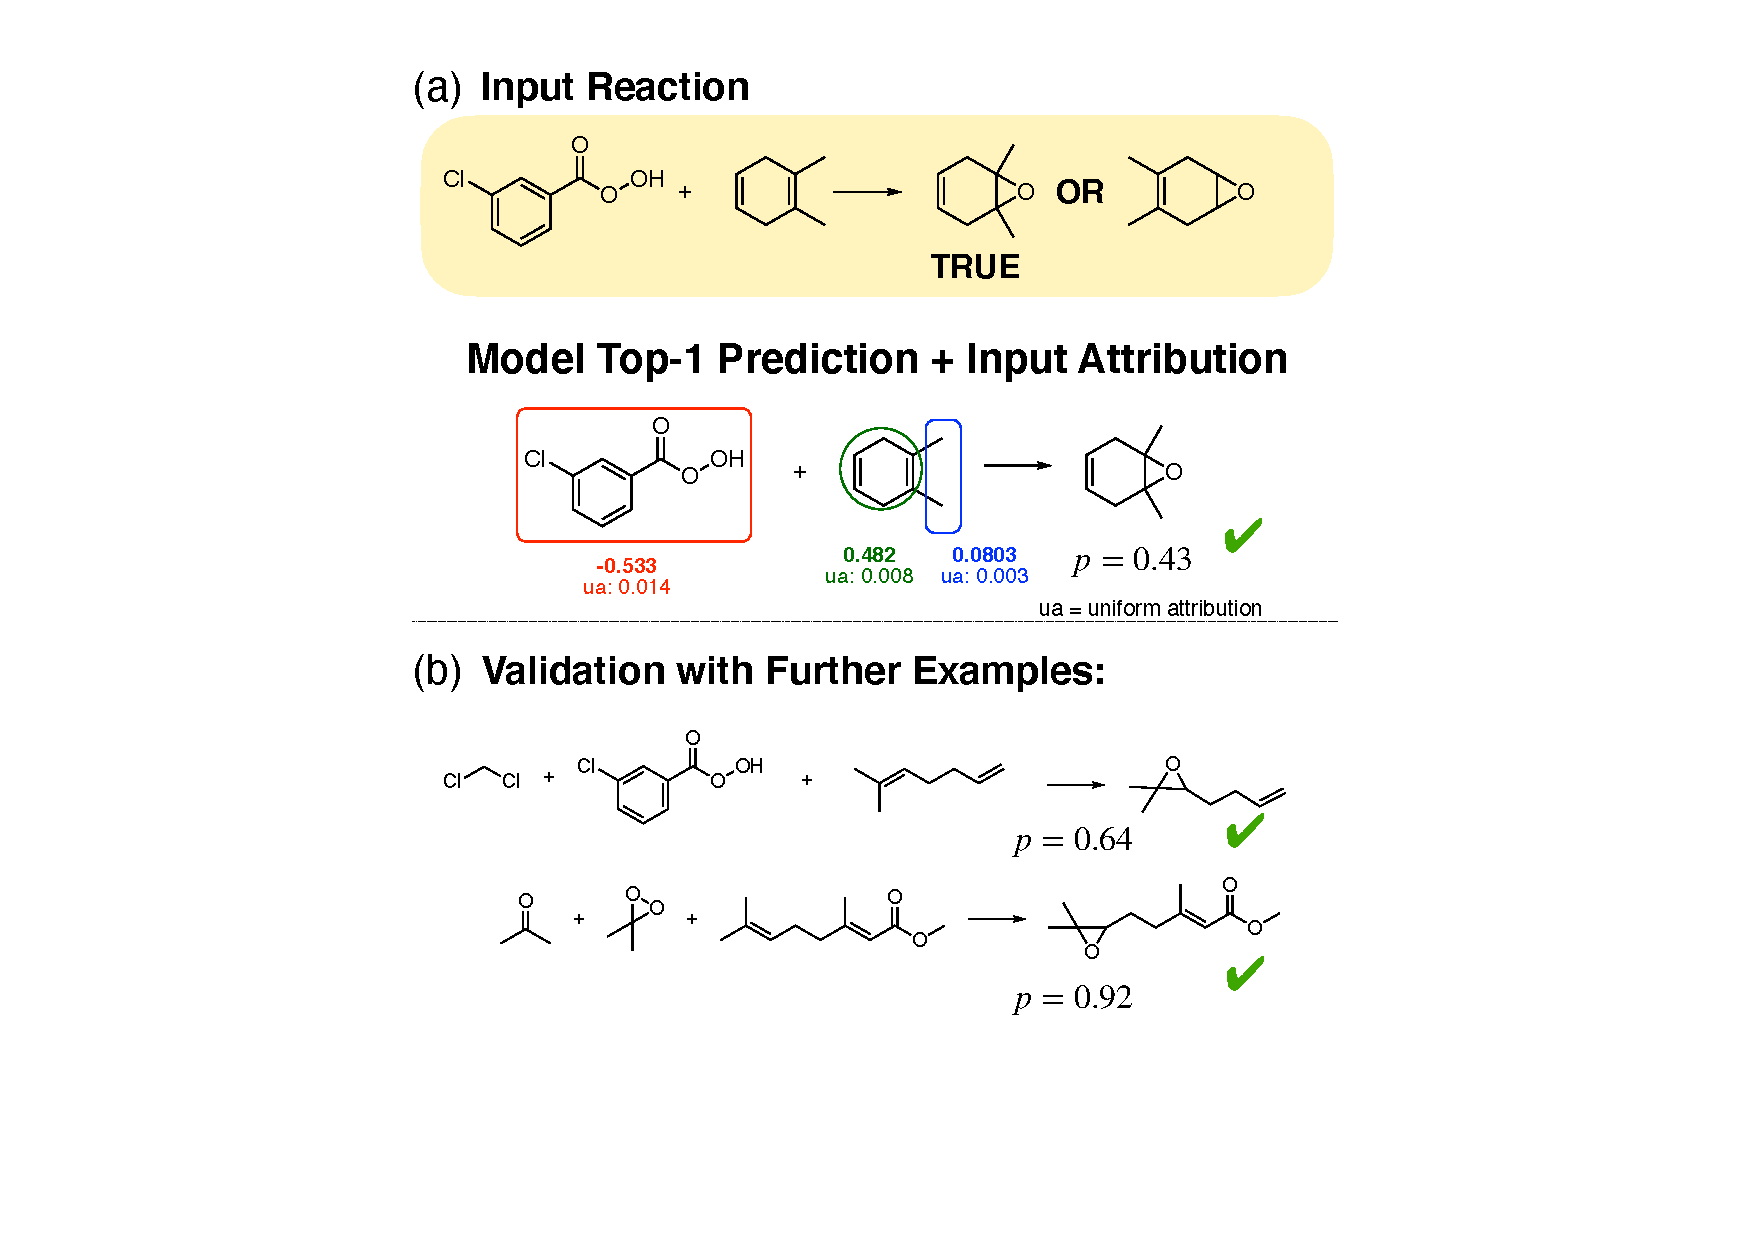
\includegraphics[width=0.6\textwidth]{Chapters/Transformer/Figs/epoxidation.pdf}
% \caption{\label{fig:epoxide} \textbf{IG attributions highlighting correct reasoning} (a) The model correctly predicts the product of a typical epoxidation reaction, and shows significant positive attributions to the two methyl group that are responsible for the selectivity. (b) We validate the model's knowledge on two unseen epoxidation reactions from chemical literature~\cite{Lluch1993}}
% \end{figure}

% The oxidation of alkenes to form epoxides is an important intermediate reaction in many synthesis plans \cite{Clayden2012}. The common oxidant in these reactions are peroxy compounds. The most widely used example of them is mCPBA, which is a versatile reagent appearing 2052 times in the USPTO dataset. This is in the high data regime where we would expect the model to do well due to the large number of different training examples available. 

% Epoxidation reactions can be regioselective, with more substituted alkenes reacting faster because they are more electron-rich \cite{Clayden2012}. A typical example reaction showing this type of selectivity is shown on Figure~\ref{fig:epoxide}(a). 

% The Molecular Transformer is able to predict the product with the correct selectivity, giving it a probability score of 0.43. The probability score of the alternative incorrect product was less only by 0.025. This is a case where the model predicts two similarly plausible outcomes, so IGs can help to judge whether or not a prediction can be trusted. Since the probability difference is close to 0, the sign of the attributions at different parts of the input is in itself interesting and contains information regarding the favoured outcome. 

% Figure~\ref{fig:epoxide}(a) shows the IG attributions of the different parts of the input.  In this case the positive attributions favour the correct product while the negative attributions favour the incorrect product. The IGs show that the two methyl substituents circled with blue are significantly contributing to the correctly predicted selectivity. The attributions on the other parts of the molecule are harder to interpret. This can be the result of the model being uncertain in the prediction leading to larger gradients along the path integral during the calculation of the attributions. 

% To validate the interpretation that the model has learnt this selectivity we generated the Molecular Transformer predictions for two further examples from the literature as shown on Figure~\ref{fig:epoxide}(b). The first example is very similar to the one examined in detail above and the model is consistently predicting the correct product. The second example is more challenging for the model for a number of reasons. First the reagent is not mCPBA but dimethyldioxirane which appears much less frequently, only 14 times in the training data, secondly both double bonds are substituted, and the difference is made by a more subtle chemistry, the ester group being electron withdrawing. The model is able to predict the correct outcome here as well confirming that the predictions are correct for the right reason. 

% \subsubsection*{Diels-Alder}

% \begin{figure}[ht!]
% 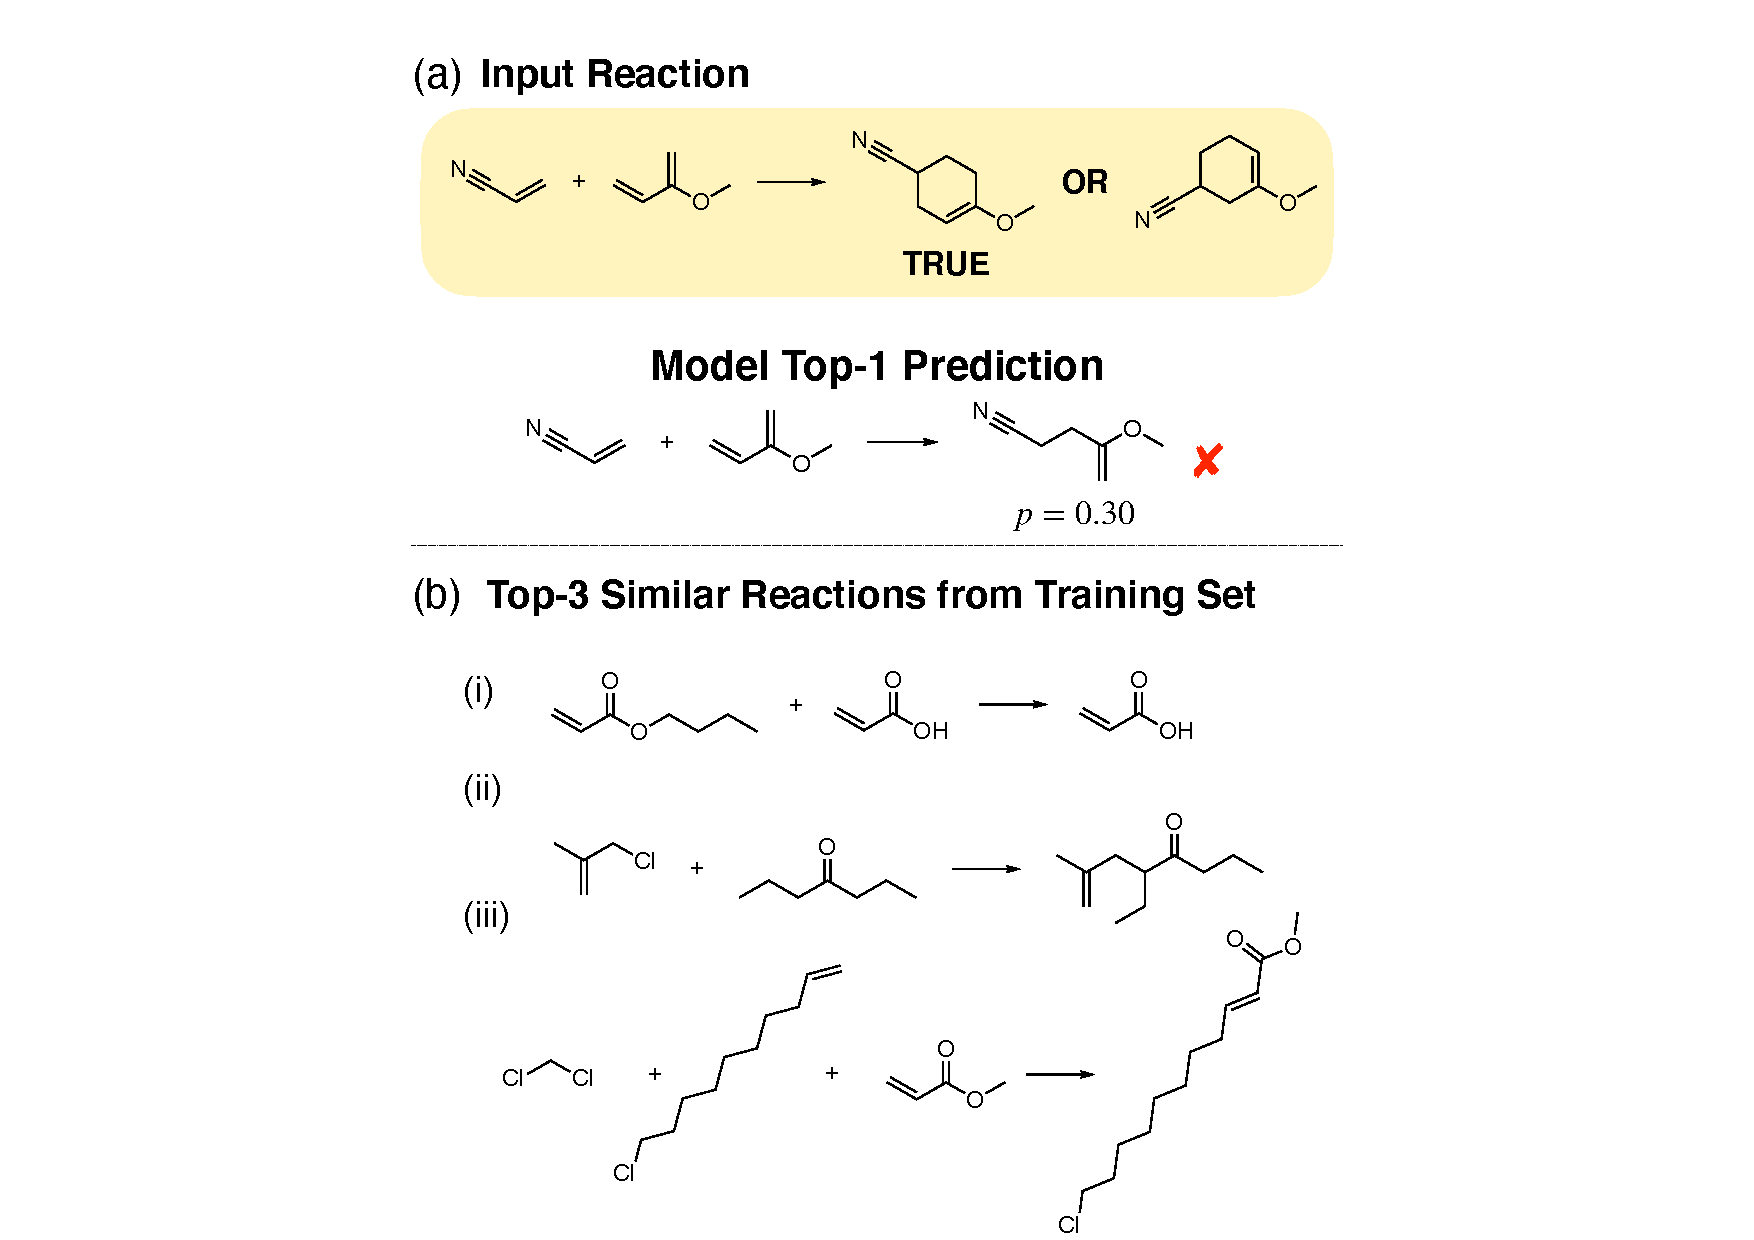
\includegraphics[width=0.6\textwidth]{Chapters/Transformer/Figs/diels_alder.pdf}
% \caption{\label{fig:diels_alder} \textbf{Data attribution explains erroneous prediction} (a) The model makes an obviously incorrect prediction on a typical example of a Diels-Alder reaction with challenging selectivity. (b) Attribution to the USPTO training data shows that the model either completely fails to recognize Diels-Alder reactions or that no Diels-Alder reaction is present in the dataset.}
% \end{figure}

% The Diels-Alder reaction transforms a conjugated diene and an alkene (called dienophile) to a six membered ring with a double bond \cite{Clayden2012}. There are very few limitations on the character of the diene. It only has to be flexible enough to take up an s-cis conformation. The dienophile, on the other hand, should have carbon-carbon double bonds conjugated preferably with an electron withdrawing group. A typical example of a Diels-Alder reaction used as a test-case is shown on Figure~\ref{fig:diels_alder}(a). 

% The Molecular Transformer was unable to predict the regioselectivity of this reaction, and in fact the predicted product was clearly wrong with the actual possible products getting 0 probability scores. Since the prediction is obviously wrong, we followed the bottom branch of the workflow at Figure~\ref{fig:workflow}(a) and generated the most similar training reactions to see what causes this erroneous prediction.

% Figure~\ref{fig:diels_alder}(b) shows the Top-3 most similar reactions from the training set based on the model encoder output similarities. The most similar training reaction (i) is an erroneous reaction, whilst the second and third are carbon-carbon bond formations, but via Grubbs methathesis \cite{grubbs} rather than cycloadditions. This means that the model has not learnt a good representation of Diels-Alder reactions in the latent space. 

% To investigate if the cause of this was a lack of training data we devised a reaction template corresponding to the [4+2] cycloaddition and found that there were only 7 reactions matching it in the entire USPTO database. This example illustrates how attribution to data can be useful for identifying erroneous predictions caused partly due to erroneous data and partly due to the scarcity of training examples. 

% \subsubsection*{Friedel-Crafts Acylation}

% \begin{figure*}[ht!]
% 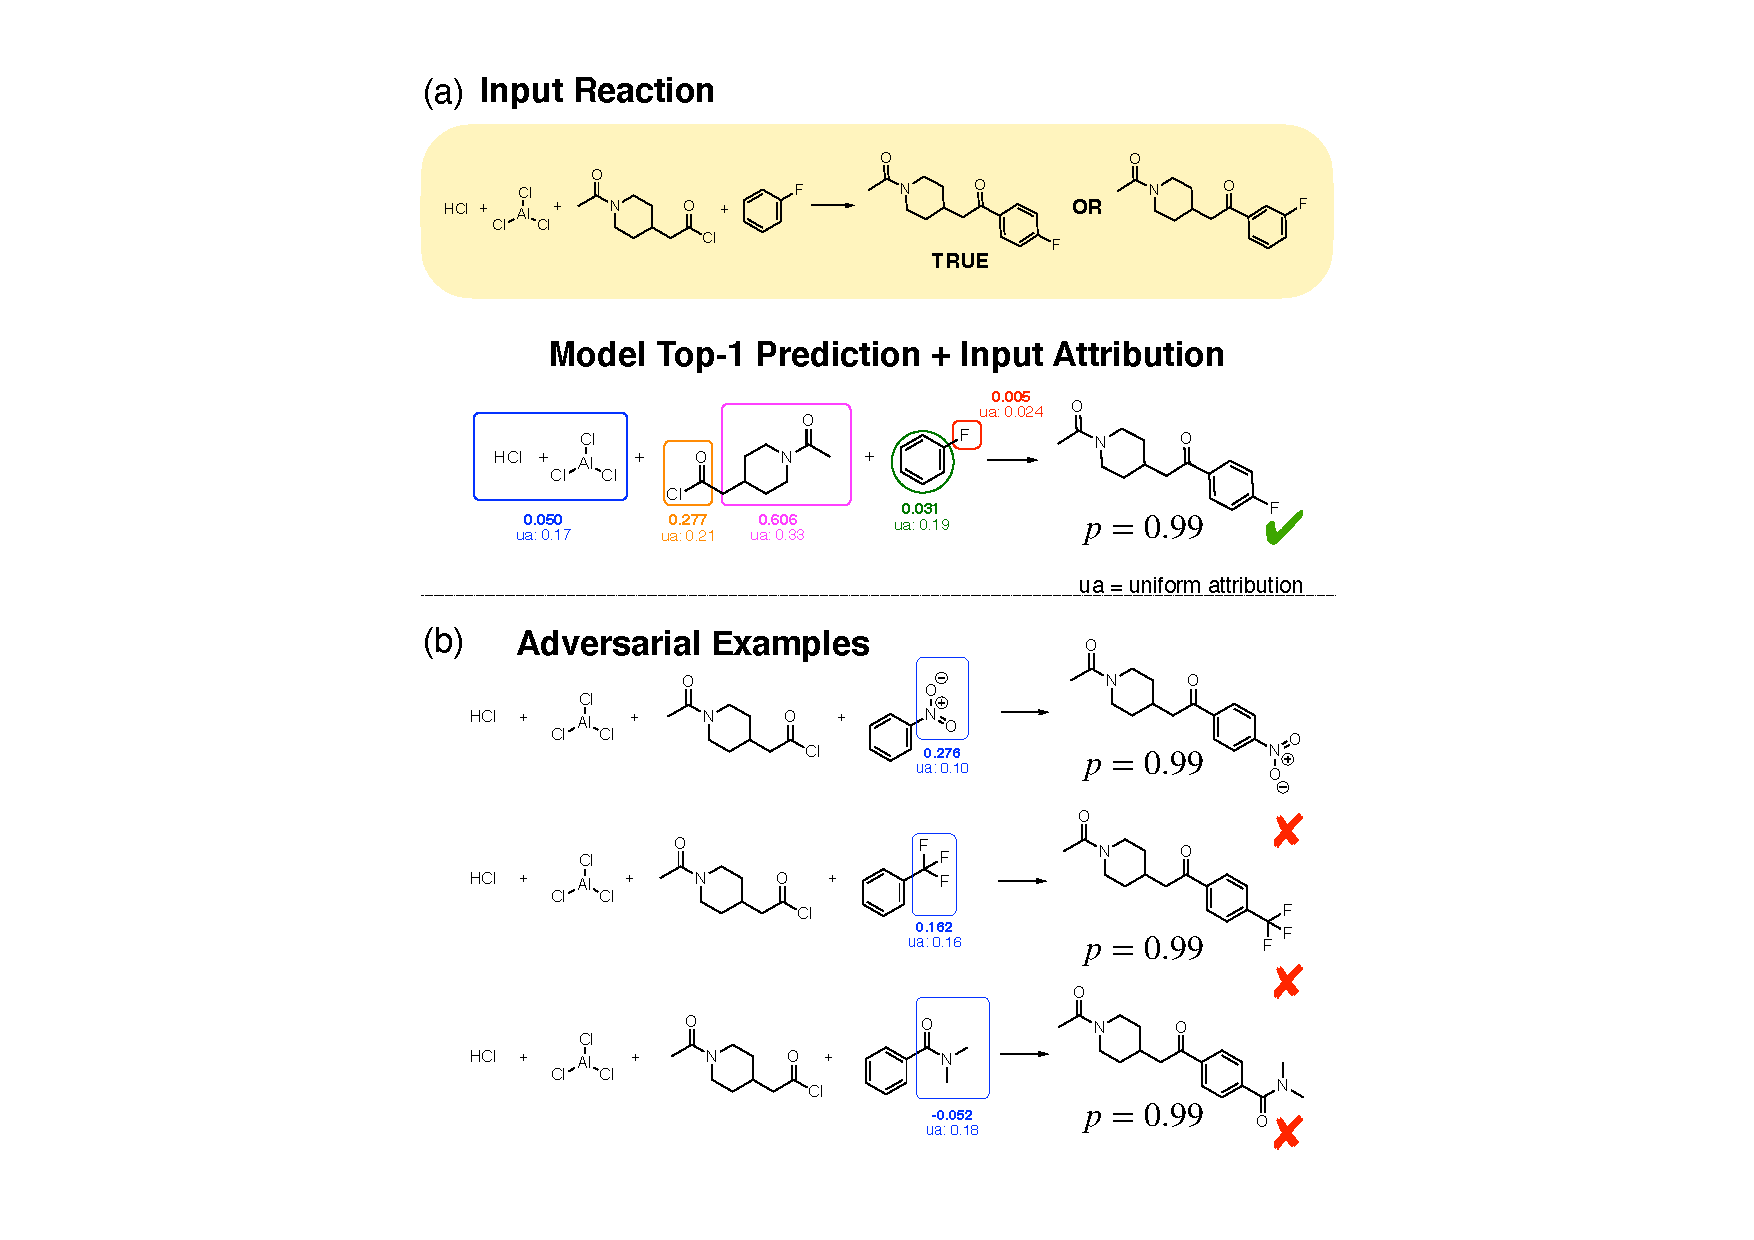
\includegraphics[width=0.6\textwidth]{Chapters/Transformer/Figs/sear.pdf}
% \caption{\label{fig:sear} \textbf{IG attributions revealing incorrect reasoning and guiding the design of adversarial examples} (a) The model correctly predicts the major para product of a typical Friedel-Crafts acylation, but low attribution is given to the para-directing -F group. (b) The model is fooled into incorrectly predicting the para product when the -F is replaced by meta-directing groups. The low attributions given to the directing groups indicate that the model has not learnt their importance.}
% \end{figure*}

% Friedel-Crafts acylation reactions are an example of electrophilic aromatic substitution \cite{Friedel1877}. In these reactions a hydrogen on an aromatic ring is substituted by an acyl group. In the case of a benzene ring with a single substituent, there are three different hydrogen positions where this substitution can happen. The electronic and steric character of the substituent on the ring determine the selectivity of these reactions. An example of a selective Friedel-Crafts reaction is shown on Figure~\ref{fig:sear}(a) where according to the patent the para product is formed with a yield of 90\% \cite{fc_para1981}. In this reaction that acyl group is primarily substituting the hydrogen in the para position compared to the -F substituent. The transformation is correctly predicted by the Molecular Transformer. 

% The IG attributions indicate that the importance of the fluorine (-F) for this reaction is completely neglected by the model. A much larger attribution is given to the reagent suggesting that the model attributes this selectivity to the reagent rather than the true directing group. Guided by the attributions we replaced the fluorine by a number of typical meta directing groups to create adversarial examples. We observe that the model (wrongly) predicts the para product. In this case negative attributions favour the meta product and positive attributions the para product. We do not find any correlation between the attribution values and the directing effect of the substituent. From this we can conclude that the model has not learnt the selectivity in the case of Friedel-Crafts acylation reactions on substituted benzene rings. 

% Interestingly in our second example the attribution on the meta directing group is negative, meaning that according to the model the amide group (correctly) favours the formation of the meta product. This agrees with chemical principles, but the model is nonetheless still predicting the para to be the major product. We hypothesize that this might be due to biases in the training data -- Figure~\ref{fig:venn_toy}(a) shows that there are many more para substitution reactions than meta in the training dataset; overlaps in the Venn diagram denotes cases where the benzene has more than 1 substituent. This could result in the model being biased towards predicting para substitutions even in the presence of meta directing groups, as the model can achieve very high (~98\%) accuracy on the training set by always predicting the para product.

% \begin{figure}[htbp!] 
% \centering    
% 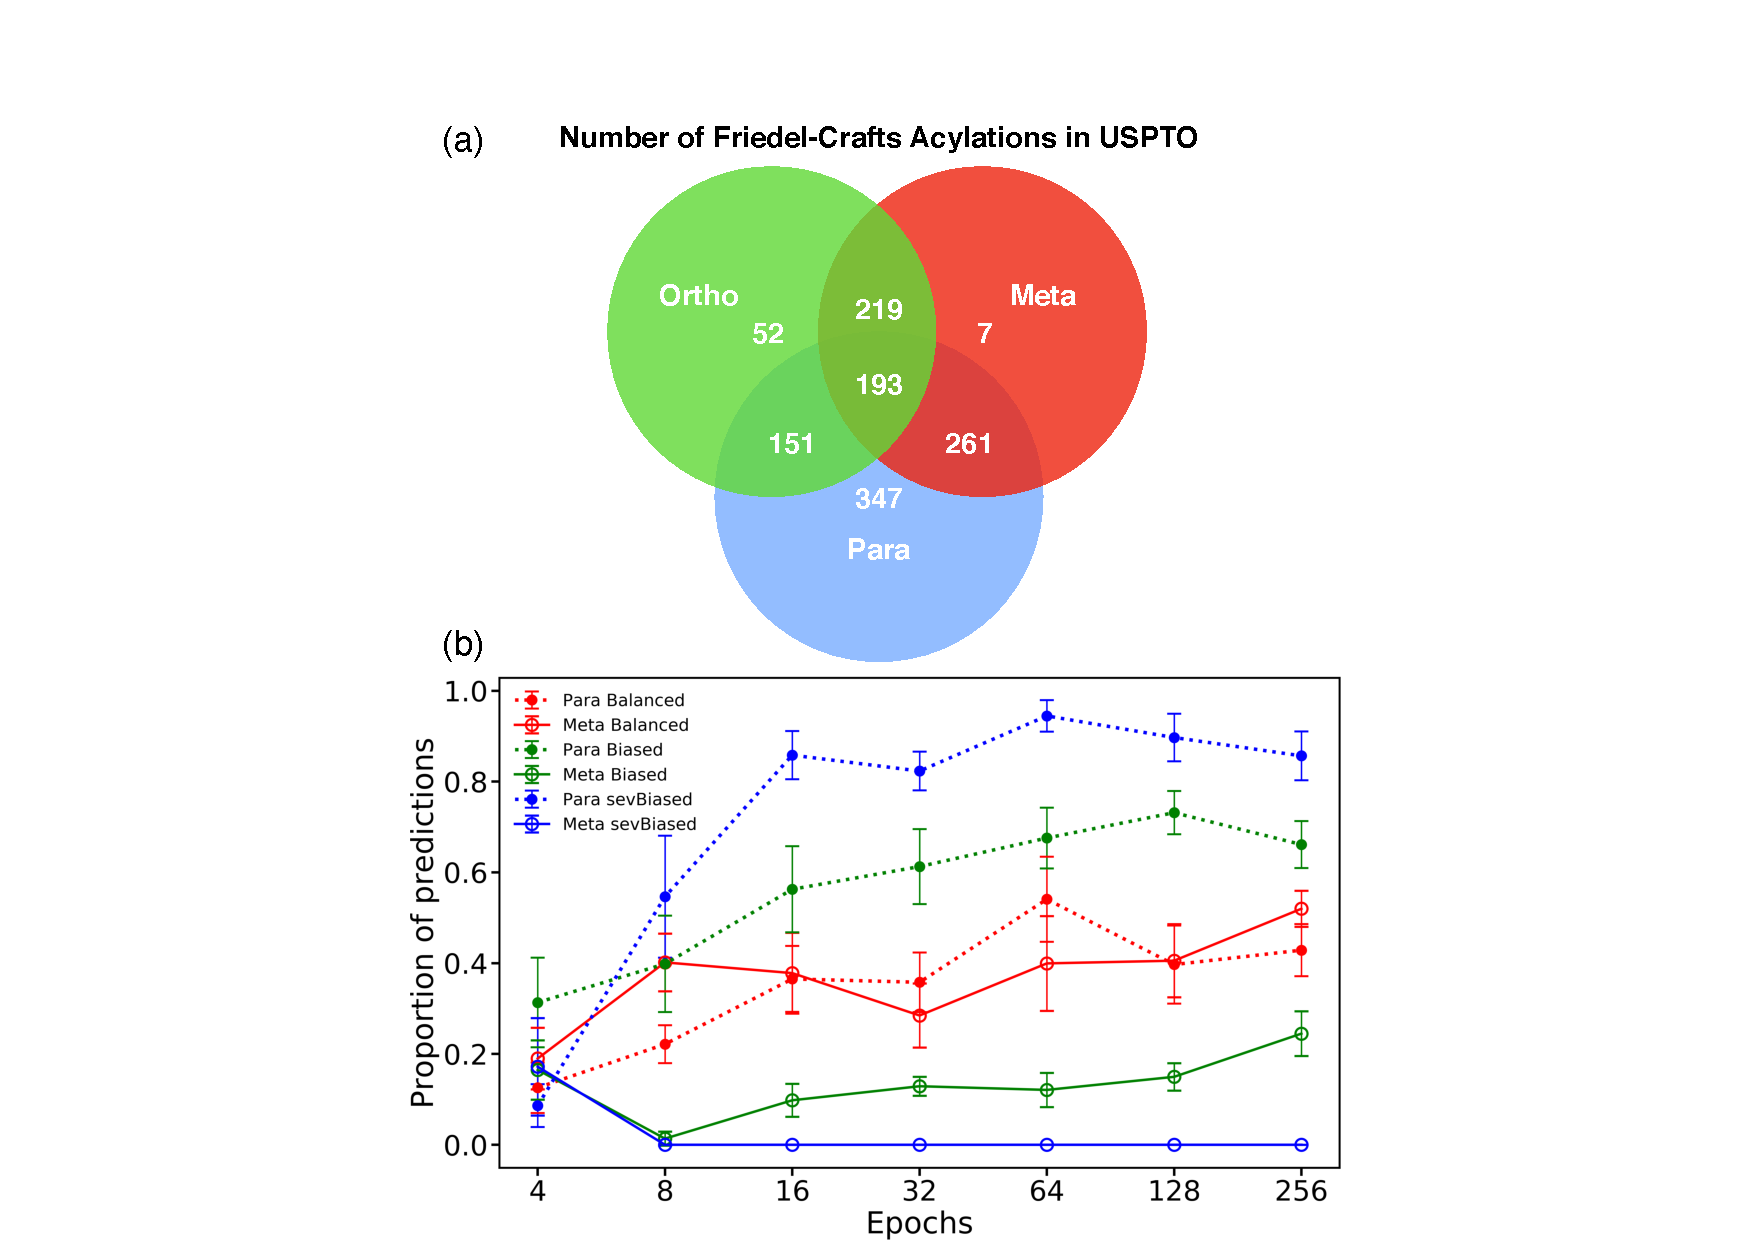
\includegraphics[width=0.6\textwidth]{Chapters/Transformer/Figs/venn_toy.pdf}
% \caption{ \textbf{The effect of biased training data on the predictions of the Molecular Transformer} (a) The number of para Friedel-Crafts acylation reactions far outweigh those of meta or ortho reactions. (b) Dataset bias is reflected in the model predictions. The figure shows the proportion of para (solid line) and meta (dashed line) predictions on a balanced test set as a function of the number of training epochs for different biased training sets. The error bars shown indicate the standard deviation in the results from training an ensemble of 10 randomly initialized models. The proportion of meta and para predictions does not always add up to 1, because it takes a number of iterations for the model to learn the SMILES syntax and we discount invalid predictions.}
% \label{fig:venn_toy}
% \end{figure}

% \subsection*{Revealing the Effect of Bias through Artificial Dataset}

% To investigate how imbalance in the training data affects the test set performance, we construct three artificial training sets using reaction templates for meta and para Friedel-Crafts substitutions. 

% The first training set is balanced, containing the same number of para and meta products. The second dataset contains 10\% meta and 90\% para products whilst the third dataset has ca 1\% meta and 99\% para products. This last ratio is closest to the ratios of the USPTO dataset. The test set for all models contains an equal number of meta and para reactions. 

% Figure~\ref{fig:venn_toy}(b) reveals that the Molecular Transformer is highly susceptible to learning dataset bias. When the model is trained on the balanced dataset, it rapidly converges to predicting equal amounts of para and meta substitution reactions, confirming that the bias is not caused by neural network architecture limitations. The model trained on the biased dataset containing only 10\% meta reactions in the training set is not able to get rid of the bias fully, but with longer training it is mitigated. For the highly biased training set the model is not able to learn to predict any meta products.

% This numerical experiment confirms that the Molecular Transformer is guilty of the Clever Hans effect -- it appears to know chemical reactivity only because it learns hidden bias in the dataset. This is analogous to the bias observed in neural machine translation, where a pronoun indicates the gender of a word, but the model disregards it when making the translation due to the presence of gender stereotypes in the training data \cite{Stanovsky2019GenderBias}. 

% \subsection*{Uncovering Scaffold bias}
% \begin{figure*}[ht!]
% 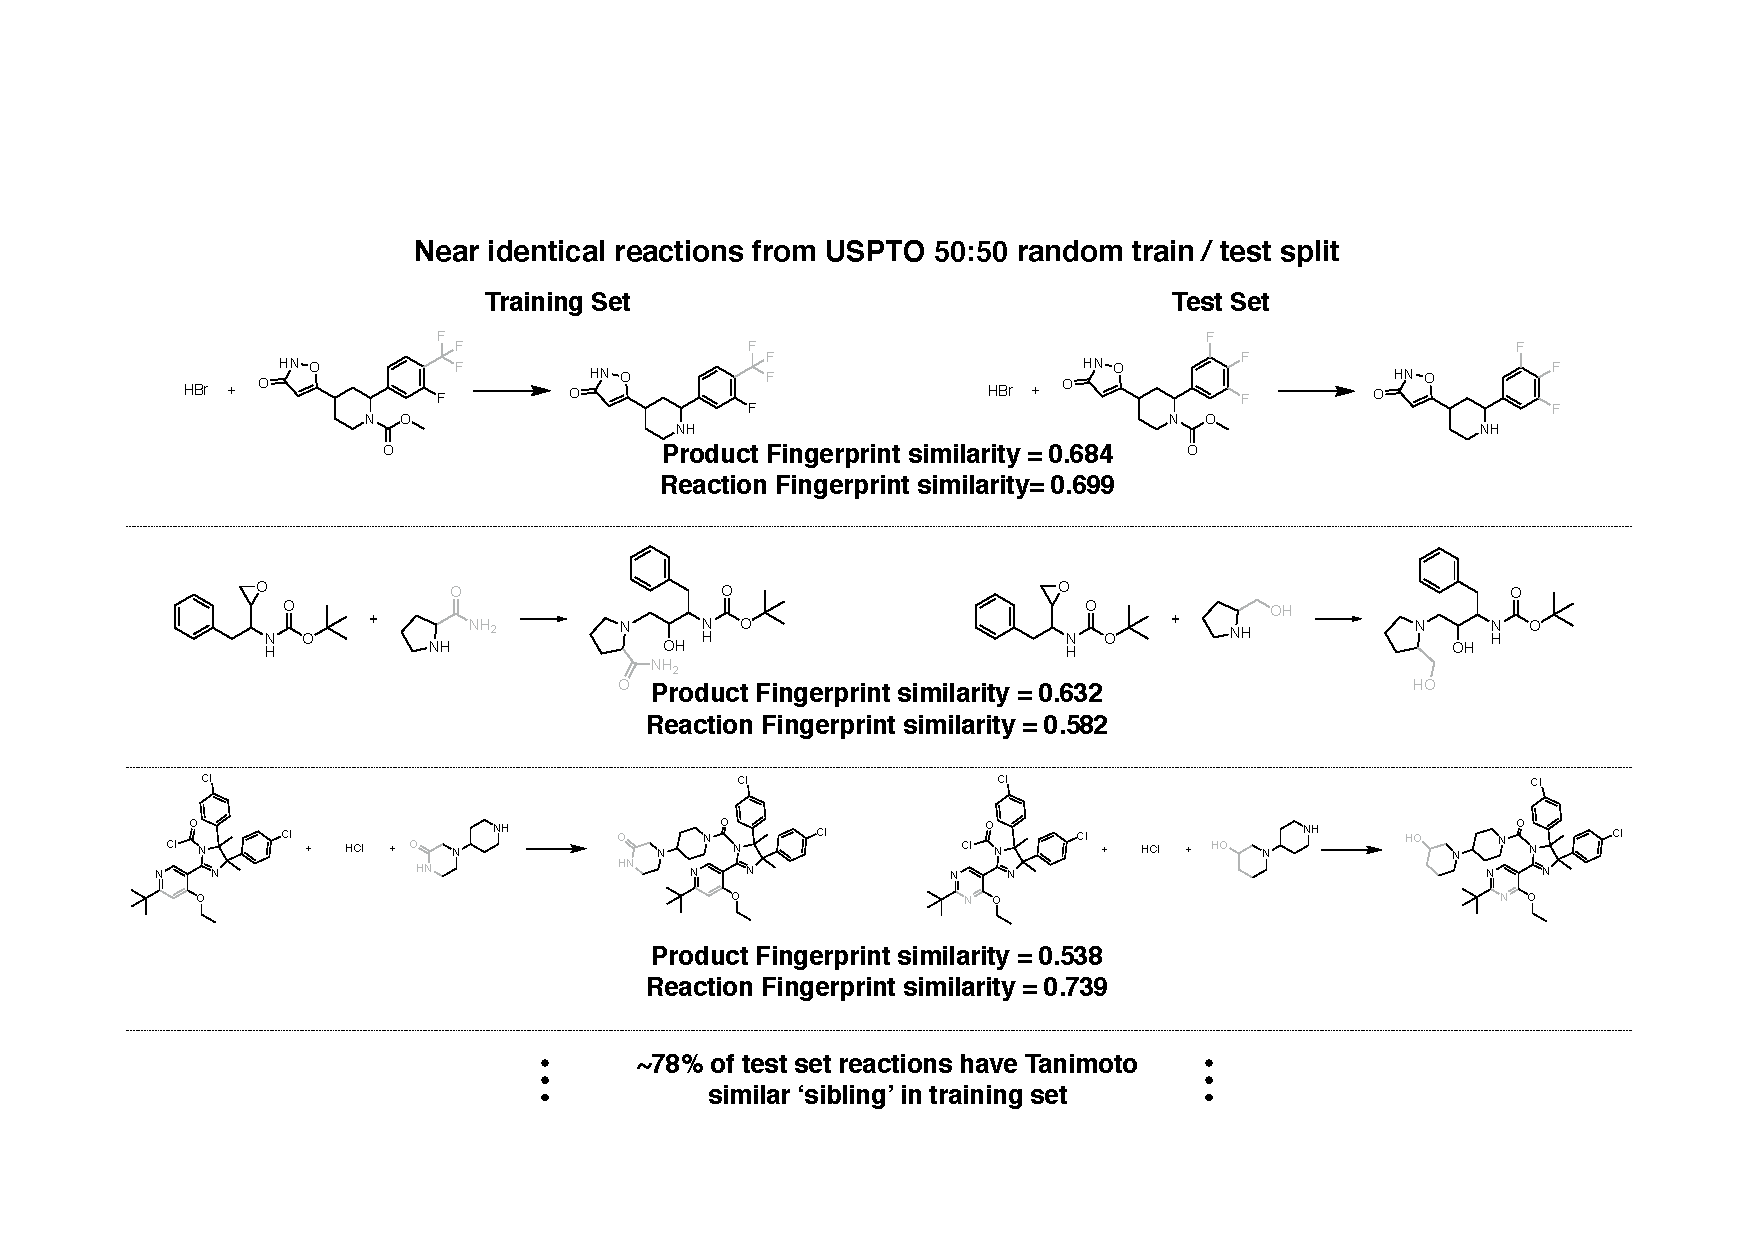
\includegraphics[width=\textwidth]{Chapters/Transformer/Figs/siblings_alt.pdf}
% \caption{\label{fig:sibling} \textbf{Near-identical training and testing reactions during random splitting of the dataset} Randomly splitting USPTO results in a large number of near-identical reactions shared between train/test sets. $78\%$ of reactions in the test set have products that are within Tanimoto similarity $0.5$ of a product in the training set following a 50:50 random split. By eye it can be seen that many reactions with similar products (differences are highlighted by shading) have similar reagents and follow near-identical reaction mechanisms. This intuition is confirmed by the similarly high similarity of the reaction difference fingerprints from the reactions. The equivalent proportions are $93\%$ and $57\%$ for Tanimoto similarity $>0.4$ and $>0.6$, respectively.}
% \end{figure*}

% Our case study of the Friedel-Crafts acylation reveals the sensitivity of the Molecular Transformer to dataset bias. We turn to examine another source of bias -- compound series bias, or scaffold bias \cite{Mayr2018compare}. This is the phenomena where very similar molecules appear in both the training and the test set. This leads to ML models achieving high accuracy on the held-out set which does not necessarily correlate with the true generalization performance of the models. This is particularly acute for drug discovery datasets as medicinal chemists typically design molecular `series' by adding various functional groups to a central chemical `scaffold'. In chemical reaction datasets, scaffold bias manifest itself as similar molecules undergoing very similar transformations.

% To gain further insight into this phenomenon, we apply a 50:50 random train/test split to the full USPTO dataset and inspect reactions from one set that have structurally similar products to those from the other set. We define the 'structural similarity' of two molecules by calculating the Tanimoto similarity $\sigma$ between the Morgan fingerprints of the respective molecules \cite{Bajusz2015Tanimoto}. Figure~\ref{fig:sibling} reveals that many training and test set reactions are remarkably similar as measured by both $\sigma$ as well as the Tanimoto similarity of the reaction difference fingerprints of the reaction \cite{Schneider2015rxnfp}.

% We find that 57\% to 93\% of reactions from the test set contain a structurally similar product to a reaction from the training set. This would not be problematic if the datapoints involved different reactants and reagents reacting via different mechanisms to form the same product. However this is not the case -- reactions with similar products often also share reactants and undergo similar chemical changes. This means that using a random train / test split to assess the performance of reaction prediction models could be a misleading indicator of their ability to generalize. Indeed, this reconciles the seeming contradiction between the reported 90\% top-1 accuracy of the Molecular Transformer and our findings above regarding the model's fragility to reactions involving chemical selectivity.

% To account for this drastic scaffold bias, we propose that datasets for training machine learning reaction prediction models should be split by the Tanimoto similarity of the reaction products. In other words, it should be ensured that no reactions in the test set have a product that is within Tanimoto similarity $\sigma$ of any product from a training set reaction. We implement this by first conducting a random split of the dataset, and then transferring all reactions that fall foul of the Tanimoto similarity criteria from the test set to the training set -- the proportion of the initial random split is adjusted until the desired final train/test ratio is obtained.

% The intent of such a dataset split is to remove structural bias but we must also make sure that the distribution of different reaction types in the train and test sets is still similar. This is important because we would like the test set score to reflect how well the model learnt the chemistry contained in the training set and we are less interested in extrapolation to unseen reaction types. To characterize the new Tanimoto-split dataset we used open-source template extraction code~\cite{Coley19WLDN5} and we inspected the distribution of reaction types in both the training and test sets for the case of the random and Tanimoto-split datasets (see Supplementary Note 1). We find that the distribution of reaction templates is not substantially perturbed and for both random and Tanimoto-splits there are no reaction templates present in the test set that are not contained in the training set, i.e. all reaction types in the test set are 'seen' by the model during training. In fact, Tanimoto-splitting increases the number of unique templates in the test set from $\sim$3k to $\sim$4.9k, suggesting that this splitting method can produce test sets that better represents the distribution of reaction types from the full dataset ($\sim$26k templates) compared to a random split. This is similar to an importance sampling scheme that helps sampling the tails of the distribution as well.

% We apply this technique to USPTO with $\sigma = 0.6$ and $\sigma = 0.4$, and train the Molecular Transformer on these two datasets. We also train the WLDN5 model of Coley et. al.~\cite{Coley19WLDN5} which is a widely-used graph-based machine learning reaction prediction model. This model explicitly represents molecules as graphs and considers reactions as series of graph edits instead of the Molecular Transformer's text-based translation of SMILES strings. 

% Table~\ref{table:tanimoto} shows that the model performance of both the graph-based model and the Molecular Transformer significantly decrease upon debiasing the dataset, but Molecular Transformer continues to outperform WLDN5.  These results show that scaffold bias affects both graph-based and sequence-based models, confirming that this bias is intrinsic to data and independent of model architecture. Importantly, this demonstrates that there is significant scope for improvement in the performance of reaction prediction, and that the 90\% accuracy obtained for a randomly split dataset does not necessarily translate to real-life applications.

% \begin{table}[!h]
% \caption{ \textbf{Evaluation of reaction prediction models on different train-test splits} The performance of the best ML models on various USPTO train/test splits are shown. The accuracy of the best-performing model is highlighted in bold.}
% \centering
% \label{table:tanimoto}
% \begin{tabular*}{0.6\textwidth}{l@{\extracolsep{\fill}}rrr}
% \toprule
%     \textbf{Model} & \textbf{Top-1[\%]} & \textbf{Top-3[\%]} & \textbf{Top-5[\%]}\\ 
%     \midrule 
% & \multicolumn{3}{c}{Original} \\
% \midrule
% Molecular Transformer & \textbf{90.4\%} & \textbf{94.6\%} & \textbf{95.3\%}  \\
% WLDN5 & 85.6\% & 92.8\% & 93.4\%  \\
% \midrule 
% & \multicolumn{3}{c}{Tanimoto Similarity \textless\,0.6} \\
% \midrule
% Molecular Transformer & \textbf{80.9\%} & \textbf{88.2\%} & \textbf{89.6\%}  \\
% WLDN5 & 75.9\% & 86.2\% & 88.8\%  \\
% \midrule
% & \multicolumn{3}{c}{Tanimoto Similarity \textless\,0.4}\\
% \midrule
% Molecular Transformer & \textbf{74.6\%} & \textbf{82.9\%} & \textbf{84.5\%} \\
% WLDN5 & 69.3\% & 80.9\% & 84.1\% \\
% \bottomrule
% \end{tabular*}
% \end{table}

% \section*{Discussion}
% We developed a framework for quantitatively interpreting the predictions of Molecular Transformer, a state-of-the-art model for predicting the outcome of chemical reactions. We show that the model makes predictions based on patterns it recognizes and the statistics of the training data, but this does not necessarily coincide with the underlying chemical drivers of reactivity. This can result in erroneous predictions. Attributing the predicted probability to parts of the input allowed us to foresee these failure modes. 

% Through this interpretation framework, we discover that the model is susceptible to the Clever Hans effect, where the correct outcome is reached by learning bias. For example, the dataset contains orders of magnitude more para than meta electrophilic aromatic substitution reactions, and the Molecular Transformer frequently arrived at correct test set prediction by simply memorising this fact. We believe that the inclusion of additional physical insight into models, as done in recent work incorporating explicit reaction mechanisms for reaction prediction \cite{bradshaw2019generative} and machine-learning regio-selectivity prediction \cite{guan_coley_robust}, could be an effective way of increasing model robustness against dataset bias. A possible way to accomplish this in Transformer models is via the augmentation of token embeddings with physical descriptors. Moreover, future efforts should focus on benchmarking other graph-based synthesis prediction tools such as the recent MEGAN architecture as well \cite{sacha2020molecule}.

% We have also shown that incorrect predictions can be the result of erroneous training data points. This can be revealed using our method to attribute model predictions to training data. This method can also aid experimental chemists using the Molecular Transformer. The references corresponding to the most similar training reactions can be used to impute experimental conditions. This principle can be used in many scientific machine learning applications where the training data is generated via text-mining which is known to lead to loss of important meta data, like reaction conditions. 

% Finally we have shown that scaffold bias is a phenomena present in the published literature on reaction prediction. Many of the reactions in the test set have almost identical twins in the training set. This leads to an overestimation of the generalization performance of the models as reported in the literature. We have re-trained two of the leading models the Molecular Transformer and the graph-based WLDN5 model on our new Tanimoto-split dataset and found that the Top-1 accuracy of the models dropped significantly.

% Our work highlights the importance of understanding and evaluating scientific machine learning models beyond looking at their accuracy on standard benchmark datasets. By rigorously applying interpretability techniques, we reveal how systematic weaknesses of the models can be uncovered, proving insights that facilitate the work of model developers. We believe further work into the use of input attribution and interpretability tools to critically analyse machine learning models for retrosynthesis, as well as other areas of computational science, is vital and necessary for continued refinement of predictive models.

% \section*{\label{sec:methods}Methods}

% \subsection*{Input attribution}
% To unpack the Molecular Transformer we decided to focus our efforts on reactions containing selective chemical transformations which means that they have multiple plausible outcomes. These reactions are most fit for identifying if the model is making the predictions on true chemical basis because the underlying chemical causes are well established. Our general framework of interpreting chemical reactions is shown on Figure~\ref{fig:workflow}(a). \par
% Once a suitable chemical reaction with two possible target molecules is chosen the Molecular Transformer probability scores of the products are generated. The difference in probability score between the true and the incorrect but plausible products is than attributed back to the reactant reagent inputs. \par
% Recently there were many methods developed and applied successfully for attributing the predictions of neural networks to parts of the input. Some of the most notable examples are LIME, SHAP, Layer-wise Relevance Propagation (LRP) and Integrated Gradients \cite{Ribeiro2016WhyClassifier, Lundberg2017APredictions, Montavon2018MethodsNetworks, Sundararajan2017}. These methods are designed to propagate back the output of the models in a fair way to determine the contribution (importance) of each of the input features to the prediction. There are several methods that have their roots in cooperative game theory and are proven to yield fair attributions as defined by the axioms of fairness \cite{Sundararajan2017}. For machine learning models where the gradients are not readily available, there are so called Shapley-values and the closely related SHAP method \cite{Lundberg2017APredictions}. For models such as the Transformer where the gradients are easy to evaluate the Integrated Gradients (IGs) method is a more natural choice \cite{Sundararajan2017} though other methods such as LRP have also been applied successfully \cite{Karpov2020}. The IGs method has also been applied previously for interpreting language models in natural language processing applications and for designing adversarial examples in the context of question answering \cite{mudrakarta2018did}. A graphical illustration of IGs is shown on Figure~\ref{fig:workflow}(b). Our approach builds on the work of McCloskey et.\,al.\,\cite{McCloskey2019} who used IGs to understand binding prediction by graph neural networks on artificial datasets. We extend the method to Transformer architectures, and use it in the context of reaction predictions on real experimental data. \par
% IGs are calculated by evaluating the path integral of the gradient of the output with respect to the input along a straight line path in the input space from a non-informative baseline to the input of interest. \par
% Given a neural network denoted by the function $F:\mathbb{R}^n\to [0,1]$, the input $x\in\mathbb{R}^n$ and the baseline input $x'\in\mathbb{R}^n$ the IG attribution of feature $i$ is given by

% \begin{equation}
% \label{eqn:IG}
%     \textrm{IG}_i(x) = (x_i - x_i') \int_{\alpha=0}^1 \frac{\partial F(x' + \alpha(x-x'))}{\partial x_i} d\alpha
% \end{equation}

% In the case of the Molecular Transformer $x$ is the $ N\times 256$ dimensional embedding of the input SMILES string of length $N$ and $x'$ is the embedding of the \texttt{'.'} token taken $N$ times. This token is used in the SMILES language to separate different molecules and hence on its own bears no chemical information making it an ideal baseline choice. To obtain the total contribution of each of the input tokens the attributions are summed along the 256 dimensional embedding vectors. \par
% Finally to make the attributions easier to interpret we devised a few simple rules to map the token level attributions to chemically meaningful substructures. Reagents like sulphuric acid or meta-Chloroperoxybenzoic acid (mCPBA) are fed into the model by their full SMILES strings but in reality they act as single units as far as the reaction is concerned. Their attributions are more meaningful to look at as a whole rather than token by token. A related problem is with the attributions corresponding to special characters in SMILES like numbers or parentheses. To resolve this we consider rings as single units and their attribution is calculated by summing over the ring atoms and numbers. This way the information about the relative positions of the ring substituents will also be included in the attribution of this part of the structure. Branches are also considered as single units and their attribution is the sum over their atoms and the parentheses specifying them. \par
% For the attributions to be meaningful it is important to look at reactions where there are two possible products which have non-zero probability scores according to the model. This is crucial since for the prediction of a single product every token of the reactant is important, since missing a remote carbon would also result in a wrong prediction. By looking at the probability difference of two plausible products this effect can be eliminated and the attributions highlight the groups driving the chemical selectivity (according to the model). In particular, canonical SMILES for both products should be used to ensure the probability scores are non-negligible.\par 

% Finally, to determine if a particular group is important according to the model we compare its attribution to the attribution that would fall onto it, if the probability difference was distributed evenly across the input tokens. Substructures that get substantially higher attribution than uniform are most important for the model when it favours one product over the other.\par

% \subsection*{Training data attribution}
% Attributing the predictions of neural networks to training data can serve as a tool for explaining predictions as well as gaining understanding of the models inner workings \cite{tetko2002}. In cases when a model predicts something very unexpected to humans attributions to parts of the input can be difficult to make sense of. Sometimes it can be much more illustrative to see a couple of example inputs that the model finds similar. Usually seeing a number of similar examples can help humans identify patterns that may serve as the basis of the model's prediction. This can either result in the discovery of new trends or laws in the scientific domain or it can reveal biases that the model has learnt. In the latter case this information can be used to improve the model or the dataset.\par
% To create a successful method for attribution to data the most crucial element is the careful design of a similarity measure. The similarity should be defined such that it measures how similar two input datapoints are according to the model. For different neural network architectures different choices of similarity measures can be appropriate. In the case of feed-forward or convolutional architectures a natural choice is to define a fingerprint vector for each data point that consists of the neural networks layer outputs (activations) concatenated together. This similarity measure has been shown to be useful for judging the reliability of toxicity models predictions by comparing molecules not in the training set \cite{Allen2020}. In the case of the Molecular Transformer which has an encoder-decoder architecture the output of the encoder layers can be used as a basis for comparing data points. Since the encoder hidden states have a non-fixed length we take the average of them across the input tokens to obtain a fixed-length $256$ dimensional vector representation for each of the reactions. Averaging is expected to work because of the relatively large dimensionality of the latent space. The size of the vocabulary of the USPTO dataset is 288 so there are almost as many orthogonal directions in the latent space as there are possible different input tokens. This is expected to lead to minimal loss of information upon averaging. For each reaction in the training set the 256 dimensional hidden state vector is generated and the matrix of training set reaction hidden states is saved as a binary. When a new example input is given to the model it is passed through the Transformer encoder and the average hidden state vector of it is calculated. A schematic diagram depicting the method is shown on Figure~\ref{fig:workflow}b. The similarity score of the input reaction vector \textbf{u} to a training set vector \textbf{v} is calculated by
% \begin{equation}
%     \textrm{score}(\textbf{u},\textbf{v}) = \frac{1}{1 + \|\textbf{u} - \textbf{v} \|}
% \end{equation}
% The top-$n$ most similar reactions from the training set are returned. 

% \subsection*{Training data}
% The training data used in this study was obtained by the text mining work of Lowe \cite{Lowe2012}. He extracted the organic reactions from US patents filed between 1976 and 2016. The dataset was filtered by Jin et. al. \cite{Jin2017} to remove duplicates and some of the erroneous reactions which resulted in a set of ca 480 000 organic reactions. This dataset though much cleaner, it still contained a large number of erroneous reactions whose sole product were halogen ions, nitric, sulphuric or phosphoric acids etc. We found that if these reactions are present in the training set the Molecular Transformer is learning them resulting in catastrophic overfitting and unchemical predictions in some cases. To eliminate this effect we deleted a further ca 8 000 reactions to obtain a dataset of 471 791 reactions. We used 377 419 for training, 23 589 for validation and 70 765 as a hold-out test set. The training set was augmented by an equal number of random equivalent SMILES strings following the protocol of Schwaller et. al. \cite{Schwaller2019}. We trained a Molecular Transformer model as described in the original paper and were able to achieve 88.8\% Top-1 accuracy on the test set, similarly to the original paper. This model was used throughout the interpretability experiments. \par
% An important aspect of the training data is that since it was extracted from patented reactions it naturally contains a number of biases. Firstly there are no negative results included meaning that any combination of reactants and reagents in the dataset leads to a well defined product. This is in contrast to reality where often there is no reaction, or the product is a mixture of many different compounds. This bias will always be reflected in the machine learning models predictions. A further bias stems from the distribution of reaction types in the dataset. Most of the patented reactions come from the medicinal chemistry community leading to reactions popular amongst medicinal chemists being over-represented. This bias can be useful since the model learns the kind of reactions medicinal chemists like using \cite{Bjerrun2020} but it also hinders generalization because popular reactions are not necessarily better as has recently been shown in the case of inorganic chemical reactions \cite{Jia2019}.

% \subsection*{Generation of the artificial dataset}
% To investigate how bias in the training data affects the Molecular Transformer we generated an artificial dataset of electrophilic aromatic substitution reactions using SMART templates. Each reaction consists of a benzene ring singly substituted with a directing group reacting with an acyl chloride to form either a para- or meta- acylated product. 

% Ten benzyl compounds with para directing groups (fluorobenzene, chlorobenzene, isopropylbenzene, tert-butyl\-benzene, N-phenylacetamide, N-phenylpropionamide, phenol, ethoxybenzene, isopropoxybenzene, sec-butyl\-benzene) and ten benzyl compounds with meta directing groups (N,N,N-trimethylbenzenaminium, (trifluoromethyl)benzene, benzaldehyde, acetophenone, methyl benzoate, ethyl benzoate, benzonitrile, nitrobenzene, methyl benzenesulfonate, ethyl benzenesulfonate) were used. The -R groups for the acyl chlorides were generated by enumerating straight carbon chains of length 2-8 with 0-1 C=C double bonds also using SMARTS templates. Acyl chlorides were obtained by placing an acyl chloride group onto a random sp3 carbon on each of the -R groups. The acyl chlorides are enumerated with the benzyl compounds to generate valid chemical reactions. 

% We vary the proportion of para:meta reactions in the training dataset and observe how the Molecular Transformer performs on a test set with an 1:1 proportion of para:meta reactions. We construct a `Balanced' dataset which has a 1:1 ratio of para:meta reactions (3100:3100) by enumerating all acyl chlorides with all benzyl compounds.  We also create a `Biased' dataset which has a 9:1 para:meta ratio (2790:310) by performing a 10:1 random split on the acyl chlorides so that less meta reactions are present. Finally we generate a `Severely Biased' dataset with 100:1 para:meta ratio (3000:30), which is closest to the observed ratio in USPTO, by performing a 33:1 random split on the acyl chlorides and also only keeping three meta-directing benzyl compounds (benzaldehyde, (trifluoromethyl)benzene, and nitrobenzene).

% The test set has an equal proportion of para and meta reactions generated using the three meta directing benzyl compounds from the `Severely Biased' training set and three para directing ones (Fluorobenzene, N-phenylpropionamide, and ethoxybenzene), together with -R groups from enumerating straight carbon chains of length 9-10 with no double bonds. This resulted in a test set with 177 para and 177 meta reactions.

% \subsection*{Tanimoto-Splitting USPTO}
% Morgan fingerprints of radius 3 with 1024 bits were used to featurize the reaction products from USPTO. For the $\sigma=0.6$ splitting, the initial dataset was randomly split 70\%:30\% and the ratio after Tanimoto splitting was 89.1\%:10.9\%. For the $\sigma=0.4$ splitting, the initial dataset was randomly split 30\%:70\% and the ratio after Tanimoto splitting was 91.7\%:8.3\%. 

% \subsection*{Data Availability}
% The USPTO dataset used to train the machine learning models is publicly available \cite{Lowe2012, Jin2017}, and Tanimoto similarity-based train/test splits of USPTO can found in the GitHub repo \href{https://github.com/davkovacs/MTExplainer.git}{MTExplainer}.\\

% \subsection*{Code Availability}
% All code used for implementing the attribution tools for the Molecular Transformer, generating the artificial Friedel-Crafts dataset, and Tanimoto-splitting USPTO can be accessed in the GitHub repo \href{https://github.com/davkovacs/MTExplainer.git}{MTExplainer}. The transformer implementation was built on top of the OpenNMT-py package.  \\

% % TODO - add SI figs

% % \section{Introduction}
% % \label{sec:int}
% % Although the design of drug candidates is exhaustingly difficult, it is in fact the `make' part of the design-make-test cycle which is the most costly, time consuming and labour intensive. The key to streamlining molecular synthesis is in improving route planning, developing faster ways of designing shorter reaction paths from basic molecular building blocks to the desired molecule, reducing the number of steps and hence the risk of failure.

% % Once a synthesis route is designed it is important to validate each step of the plan. Forward chemical reaction prediction is concerned with predicting the (major) product of an organic reaction given the reactants, reagents and preferably the conditions like solvent, temperature, concentrations etc. By having the ability to predict the product of reactions with reliable uncertainties it is possible to design clever synthesis plans where the reactions with higher uncertainty are put first. This way if a synthesis protocol fails it does so fast and cheap instead of in the later stages of the route where substantial time and cost would go to waste.

% % Route planning and reaction prediction have traditionally been done by expert chemists relying on experience, as well as reaction databases like Reaxys \cite{ElsevierReaxysDatabase}. Nowadays, Computer Assisted Synthesis Planning tools are increasingly being used \cite{Coley2018}, as these tools can memorise libraries of commercially available building blocks and quickly evaluate large numbers of possible bond disconnections via efficient algorithms such as Monte Carlo Tree Search \cite{Segler2018PlanningAIb}. Unsurprisingly, machine learning methods have also entered into the fray \cite{Coley2019AutonomousOutlook, Coley2019AutonomousProgress} and have recently emerged as the most successful approach \cite{Coley2018, Schwaller2019MolecularPrediction}.

% % ML reaction prediction models are trained on reaction data that is extracted from patents and publications. In these documents usually the metadata about reactions like the temperature, concentrations and solvents are found in the synthesis protocol section making it very challenging to extract this information in an automated manner. Therefore these models are usually trained only on the reactants and reagents with all of the context information missing. In spite of this there are reported models achieving remarkably high near 90\% Top-1 prediction accuracy on these datasets, even outperforming quantum mechanics-based approaches \cite{Schwaller2019MolecularPrediction}. 

% % The natural question that arises is: how is the model able to achieve such high accuracy on often rather challenging reactions from such limited source of data? Has the model learnt the well-established underlying mechanistic drivers of reactivity purely from data? It is of utmost importance to validate these models to see if they are able to generalize and predict the outcome of reactions reliably or if they are merely learning hidden biases in the datasets which results in the seemingly strong performance. 

% % One way to accomplish this is with ML interpretability methods \cite{Alvarez-Melis2018OnMethods}. Interpretability methods can help uncover the reasoning of model predictions in simple well understood cases where the physical or chemical cause for certain outcomes is well established. For chemical reaction prediction our understanding of mechanisms and selectivities serves as good guides for the observed reactivities.

% % In this work, we use a well-known ML interpretation method called Integrated Gradients (IGs) to probe the understanding of the Molecular Transformer (MT), the current state-of-the-art machine learning model for chemical reaction prediction. Our approach builds on the work of McCloskey et.\,al.\,\cite{McCloskey2019UsingChemistry} who used IGs to understand binding prediction models on artificial datasets. We extend the method to Transformer architectures, and use it in the context of reaction predictions on real experimental data. We also present a novel method for attributing the predictions of neural network models to training set datapoints. With these tools we show that MT often fails to learn the mechanistic reasoning behind chemical selectivity and hypothesize that this is due to hidden biases in the dataset. We justify this claim by creating biased synthetic datasets and demonstrating selectivity bias in the model predictions, suggesting that it is the quality of training data rather than the particulars of model architectures that is constraining the potential for ML reaction prediction.

% % The work in this chapter was done collaboratively with D\'{a}vid P\'{e}ter Kov\'{a}cs. We did the code development together and discussed all of the results of the work. He executed the code, analysed the model attributions, and designed the majority of the experiments and all of the adversarial examples. I created the SMARTS templates for counting statistics from the patent datasets as well as for dataset generation in the synthetic experiments. Preliminary results from this work were presented at the ICML 2020 `ML Interpretability for Scientific Discovery' Workshop \cite{Kovacs20unpack}. All code including a \texttt{README} with the usage can be found in the GitHub repo \texttt{MTExplainer} \cite{Kovacs2020MolecularExplainer}.

% % \section{Methods}

% % \subsection{Molecular Transformer}
% % The Molecular Transformer \cite{Schwaller2019MolecularPrediction} is a tailored version of the Transformer architecture \cite{Vaswani2017} which was designed for machine translation and has had wide-ranging success in many Natural Language Processing tasks. It has an encoder-decoder structure, where both the encoder and the decoder are made up of so called transformer blocks. These blocks process the inputs by applying a multi-head scaled dot-product attention mechanism followed by layer normalization and some fully connected feed forward layers. Mathematical details can be found in (somewhere).

% % The string input to the model is broken down into individual tokens with a learnt embedding that is fed into the encoder layer with positional encoding. The encoder is composed of 4 identical attention blocks each containing a multi-head self-attention layer and a 2-layer fully connected feed-forward neural network. The decoder is very similar to the encoder with the only difference being that the multi-head attention uses the output of the encoder as the keys and the values with the output of the previous decoder layer being the query. The predictions are generated in an autoregressive way meaning that the decoder predicts one token at a time and the previously generated tokens are fed into the decoder when generating the next tokens. The prediction is considered final when an \texttt{<end>} token is generated or the maximum length is reached. Through this process each translation gets assigned a probability score:
% % \begin{equation}
% %     P(\textrm{tgt} \mid \textrm{src}) = \prod_{i=1}^N P(\textrm{tok}_i \mid \textrm{tok}_1, \cdots , \textrm{tok}{i-1}, \textrm{src}) 
% % \end{equation}
% % where $\textrm{tok}_i$ is the $i$-th predicted token and $N$ is the length of the prediction.

% % Our implementation of the work was based on the \texttt{OpenNMT} package \cite{Klein2017}.

% % \subsection{Data}
% % We trained the model on a publicly available dataset of organic reactions mined from the US patent office \cite{Lowe2012} which has been filtered \cite{Jin2017}. The data contains reactants, reagents, and products represented as SMILES (without including stereochemical information) which is a text based representation of molecules\cite{Weininger1988, Weininger1989}. The training set was made up of 377 419 reactions which we augmented by an equal number of identical reactions made up of random equivalent SMILES. This augmentation is done to help the model to learn the underlying molecular graph from the SMILES sequence.There were 23 589 reactions for the validation set and 70 765 reactions in the hold-out test set, neither of which were augmented. The SMILES strings were tokenized following \cite{Schwaller2019MolecularPrediction}.

% % The trained model achieved 88.8\% Top-1 accuracy on the test set. This model was used throughout the interpretability experiments and is referred to as USPTO Transformer.

% % The second dataset used was the commercial Pistachio dataset \cite{Mayfield2018Pistachio2.0}. This dataset contains over 9 million reactions text mined from US and EPO patents. This dataset was filtered similarly to USPTO to remove erroneous and and a large number of duplicate reactions. The final dataset consisted of 2 375 385 reactions, of which 2 019 078 were used for training, 118 770 for validation and 237 537 for testing. 

% % The model trained as described above achieved 76.4\% Top-1 accuracy on the test set. Even though this looks like a substantially lower performance in reality the two models perform similarly well on new reactions. The possible reasons for the large difference in the measured performance on the held-out test sets are described in detail below. This model obtained was also used in the interpretability experiments to test the effect of increased training set size on the models understanding of chemistry and is referred to as Pistachio Transformer from here onwards. 

% % \subsection{Integrated Gradients}
% % To understand the predictions of MT with respect to the input features, we use the Integrated Gradients \cite{Sundararajan2017AxiomaticNetworks} attribution method. Integrated Gradients (IGs) is a principled model-agnostic feature attribution method adapted from game theory which obeys certain axioms of fairness. It can be used for any model where gradients are available, which is the case for all neural networks that are trained by some variant of gradient based optimization.

% % In general, the attribution of feature $i$ for input $x$ is given by
% % \begin{equation}
% % \label{eqn:IG}
% %     IG_i(x) = (x_i - x_i') \int_{\alpha=0}^1 \frac{\partial F(x' + \alpha(x-x'))}{\partial x_i} d\alpha
% % \end{equation}
% % where $x_i$ is the vector of feature $i$ for the input $x$, and $x_i'$ is a vector corresponding to a non-informative baseline input, $F(x)$ represents the model prediction for input $x$, and the integral is taken over the straight-line path from the baseline to the input of interest. 

% % It has been discussed before that the choice of baseline can have a large effect on the values of the attributions \cite{sturmfels2020visualizing}. While we could have chosen unreactive molecules as our baseline, it is important to select baselines which are completely non-informative to avoid any ambiguity. This would traditionally be the black image in the case of image recognition. In this work we use the embedding vector of the SMILES ` \textbf{.} ' token which is used to separate different molecules and hence does not contain any chemical information on its own.

% % For MT, we take great care to define $F(x)$ as it is not an appropriate question to ask what part of the reactant-reagent input is most important for predicting a given product. All of the input tokens contain crucial information that are used by the decoder to generate the entire target structure correctly. To eliminate this effect we define $F(x)$ as the difference in predicted probability of two possible products. Since the inert parts of the input are the same for the two products they should not substantially contribute to their predicted probability difference. This method is especially suited for examining reactions with selectivities. In other words we attribute the selectivity between two products to the inputs, ideally highlighting the chemically important groups driving this selectivity (by summing the attributions of the tokens comprising these groups).

% % If it is found that the correct product is predicted for the wrong reason i.e. the attribution on the chemical important group is low, it can be confirmed that model has not been able to learn the underlying chemistry through the construction of adversarial examples. In these examples we only change the parts that are chemically important, but not according to the model. This way the model can be fooled into incorrect predictions if the interpretation is correct, or the interpretation can be falsified if the model is able to predict the correct product. This is a crucial element of our method as any interpretation that cannot be falsified would be no more than speculation.

% % When talking about the size of an attribution we always compare it to the amount of attribution the group would get if the probability difference would be distributed uniformly across the input tokens. This serves as a way of normalizing the attributions by the size of the different substructures. We consider the parts of the reactant that get substantially higher attribution than expected to be `important'.

% % \subsection{Data Attribution}
% % In cases when a model predicts something very unexpected to humans attributions to parts of the input can be difficult to make sense of. Sometimes it can be much more illustrative to attribute to data instead and see a couple of example inputs that the model finds similar, which can reveal biases that the model has learnt.

% % To successfully attribute to data, we must understand how `similar' two input datapoints are according to the model by defining a similarity metric. For the Molecular Transformer which has an encoder-decoder architecture we use the output of the encoder layers as a basis for comparing data points. The challenge lies in the fact that these encoder hidden states have a non-fixed length $256\times N$ where $N$ is the length of the input sequence. To overcome this we average these vectors over the sequence dimension $N$, obtaining a representation of fixed size 256. We hypothesized that averaging can work because of the relatively large dimensionality and hence sparsity of the embedding space, allowing the averaged vector to retain most of the information about the structure, reagents and reactivity. 

% % We generated these averaged encoder state vectors for all of the reactions in the training sets. When a new example input is given it is passed through the Transformer encoder and the average hidden state vector of it is calculated. The similarity score of this vector to the training set vectors is calculated by
% % \begin{equation}
% %     score = \frac{1}{1 + D}
% % \end{equation}
% % where $D$ is the Euclidean distance between the vectors. This can be implemented in a vectorized way resulting in very quick computation even in the case of dataset sizes like Pistachio made up of over 2 million training examples. The top-$n$ most similar reactions are returned where $n$ is defined by the user. A similar approach is used in \cite{Allen2020} to measure the model-learned similarity between molecules for a graph neural network trained on toxicity prediction. These similarities are also used as evidence for judging the reliability of the model predictions, but only for unseen molecules not in the training set. In this work we go beyond assessing reliability into explaining the failures of the model by explicitly examining the training data itself to reveal hidden biases.

% % % From each reaction type we design a representative reaction that contained some selectivity and produce predictions with the USPTO and Pistachio Transformer. In the case of correct predictions the IG attributions were generated and evaluated whether they agreed with the underlying chemical causes of selectivity or not. After that based on the IGs a number of adversarial examples were generated to either confirm that the model is making the right prediction for the right reason or to confirm that the interpretation is correct and the model did not learn the underlying chemical causes. Attributions to training data were also generated to help confirm that the model is correctly making predictions based on chemically similar examples and also to help identify the causes of incorrect predictions. The causes found include the absence of similar reactions in the training set, erroneous training datapoints and biases in the training set. 

% % \begin{figure}[htbp!] 
% % \centering    
% % 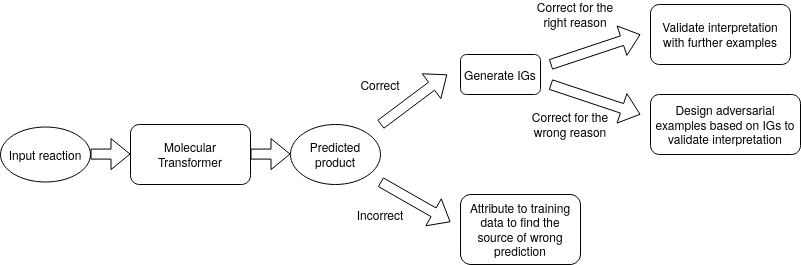
\includegraphics[width=1.05\textwidth]{Chapters/Transformer/Figs/workflow.png}
% % \caption[workflow]{An overview of the workflow for interpreting the Molecular Transformer.}
% % \label{fig:workflow}
% % \end{figure}

% % \section{Results}
% % To interpret the predictions of the Molecular Transformer we follow an analysis workflow (Fig~\ref{fig:workflow}) and examine a number of reaction types that are commonly used in synthetic organic chemistry using both input and data attribution techniques.
% % \subsection{Diels-Alder reactions}
% % The Diels-Alder reactions transform a conjugated diene and an alkene (called dienophile) to a six membered ring with a double bond \cite{Clayden2012}. A typical example is shown in Fig~\ref{fig:da1}. Diels-Alder reactions are regioselective meaning that the methoxy and nitrile group can be opposite or one carbon apart on the ring formed as shown in Fig~\ref{fig:da1}. The major product is the one marked TRUE on the figure because of more favourable HOMO-LUMO interactions. Due to the large number of possible products and complicated rules determining the major product the Diels-Alder reaction can serve as a challenging test for any reaction prediction model.

% % \begin{figure}[htbp!] 
% % \centering    
% % 
\includegraphics[width=0.9\textwidth]{Chapters/Transformer/Figs/da1.png}
% % \caption[Diels-Alder]{A typical example of a Diels-Alder reaction with challenging selectivity.}
% % \label{fig:da1}
% % \end{figure}

% % \begin{figure}[htbp!] 
% % \centering    
% % 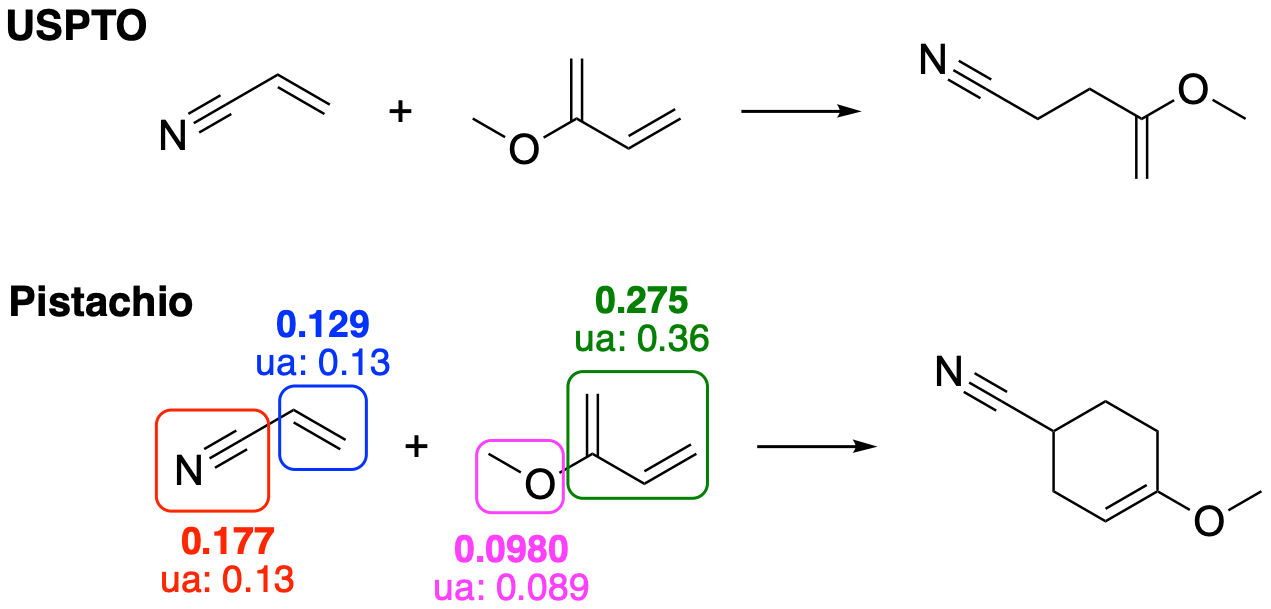
\includegraphics[width=0.8\textwidth]{Chapters/Transformer/Figs/da1_preds.png}
% % \caption[Diels-Alder]{The USPTO transformer makes a completely incorrect prediction, while the Pistachio model correctly predicts the product and recognises the importance of the nitrile group. For the Pistachio model the IG attributions are shown together with the corresponding uniform attribution (ua) values. }
% % \label{fig:da1_preds}
% % \end{figure}

% % Fig~\ref{fig:da1_preds} shows the Top-1 prediction of the USPTO and Pistachio models. The USPTO model does not seem to recognize the Diels-Alder reaction and gets the prediction wrong, indicating its own uncertainty by assigning a very low score of 0.300 to the prediction. To find the reason for the wrong prediction we attributed to training data (Fig~\ref{fig:da1_uspto_dat}). The first reaction seems to be an erroneous datapoint whereas the other two are different carbon-carbon bond formation reactions. This indicates that either the model has not learnt to recognize Diels-Alder reactions or the dataset did not contain any of them. 

% % \begin{figure}[htbp!] 
% % \centering    
% % 
\includegraphics[width=1.0\textwidth]{Chapters/Transformer/Figs/da1_uspto_dat.png}
% % \caption[Diels-Alder]{Attribution to the USPTO training data shows that the USPTO transformer either completely fails to recognize Diels-Alder reactions or that no Diels-Alder reactions exist in the dataset. }
% % \label{fig:da1_uspto_dat}
% % \end{figure}

% % To check this we devised a simple reaction template of Diels-Alder reactions and ran a template matching algorithm on the training data. We validated the template by ensuring it was able to identify the reactions where a diene and a double bond participate in cyclo-addition, which made up 80\% of the $\sim$2.3k labelled Diels-Alder reactions in Pistachio. This template matched only 7 reactions in the USPTO dataset confirming that it contains very few instances of this type of reaction. Furthermore this suggests that the model was not able to generalize across chemical space to infer this reactivity from different types of reactions. This level of generalization could only be expected from physics based models that have direct access to quantum mechanical information driving the reactions.

% % \begin{figure}[htbp!] 
% % \centering    
% % 
\includegraphics[width=1.0\textwidth]{Chapters/Transformer/Figs/da1_adv.png}
% % \caption[Diels-Alder]{Further test reactions correctly predicted by the Pistachio model, validate that Pistachio correctly understands Diels-Alder reactions. \cite{Husinec2011AnnulationsDerivatives, Tiamas2018AsymmetricChalcones}}
% % \label{fig:da1_adv}
% % \end{figure}

% % For the Pistachio model the Top-1 prediction is correct, as shown in Fig~\ref{fig:da1_preds}, and it has a confidence score of 0.819 indicating that it is fairly certain in the prediction. We also generated the IGs for this reaction to see if the selectivity is caused by the relevant nitrile and methoxy groups. The probability difference between the correct major and the minor products was 0.77 and it was distributed on the compounds as shown in Fig~\ref{fig:da1_preds} alongside the uniform attribution values. It can be seen that the nitrile group received a higher than uniform attribution indicating that the model recognises its importance. The same cannot be said unambiguously about the methoxy group whose attribution is only slightly more than the corresponding uniform value. Based on this example we can conclude that the model has learnt to recognize Diels-Alder reactions, and the IGs point towards the fact that it has learnt the regioselectivity causes too. To confirm this a couple of reactions taken from publications were tested (Fig~\ref{fig:da1_adv}) and the Pistachio transformer is able to predict the correct products. 

% % \subsection{Friedel-Crafts acylation reactions}
% % \label{subsec:friedel}
% % Friedel-Crafts acylation reactions are an example of electrophilic aromatic substitution reactions \cite{Clayden2012, Friedel1877SurEtc.} where a hydrogen on an aromatic ring is substituted to an acyl group. In the case of a benzene ring with a single substituent on it there are three different hydrogen positions where this substitution can happen. The electronic and steric character of the substituent on the ring will determine the selectivity of these reactions. An example of a selective Friedel-Crafts reaction is shown in Fig~\ref{fig:sear}. 

% % \begin{figure}[htbp!] 
% % \centering    
% % 
\includegraphics[width=0.9\textwidth]{Chapters/Transformer/Figs/sear.png}
% % \caption[FC]{Friedel-Crafts acylation reaction taken from the USPTO training set showing para selectivity.}
% % \label{fig:sear}
% % \end{figure}

% % \begin{figure}[htbp!] 
% % \centering    
% % 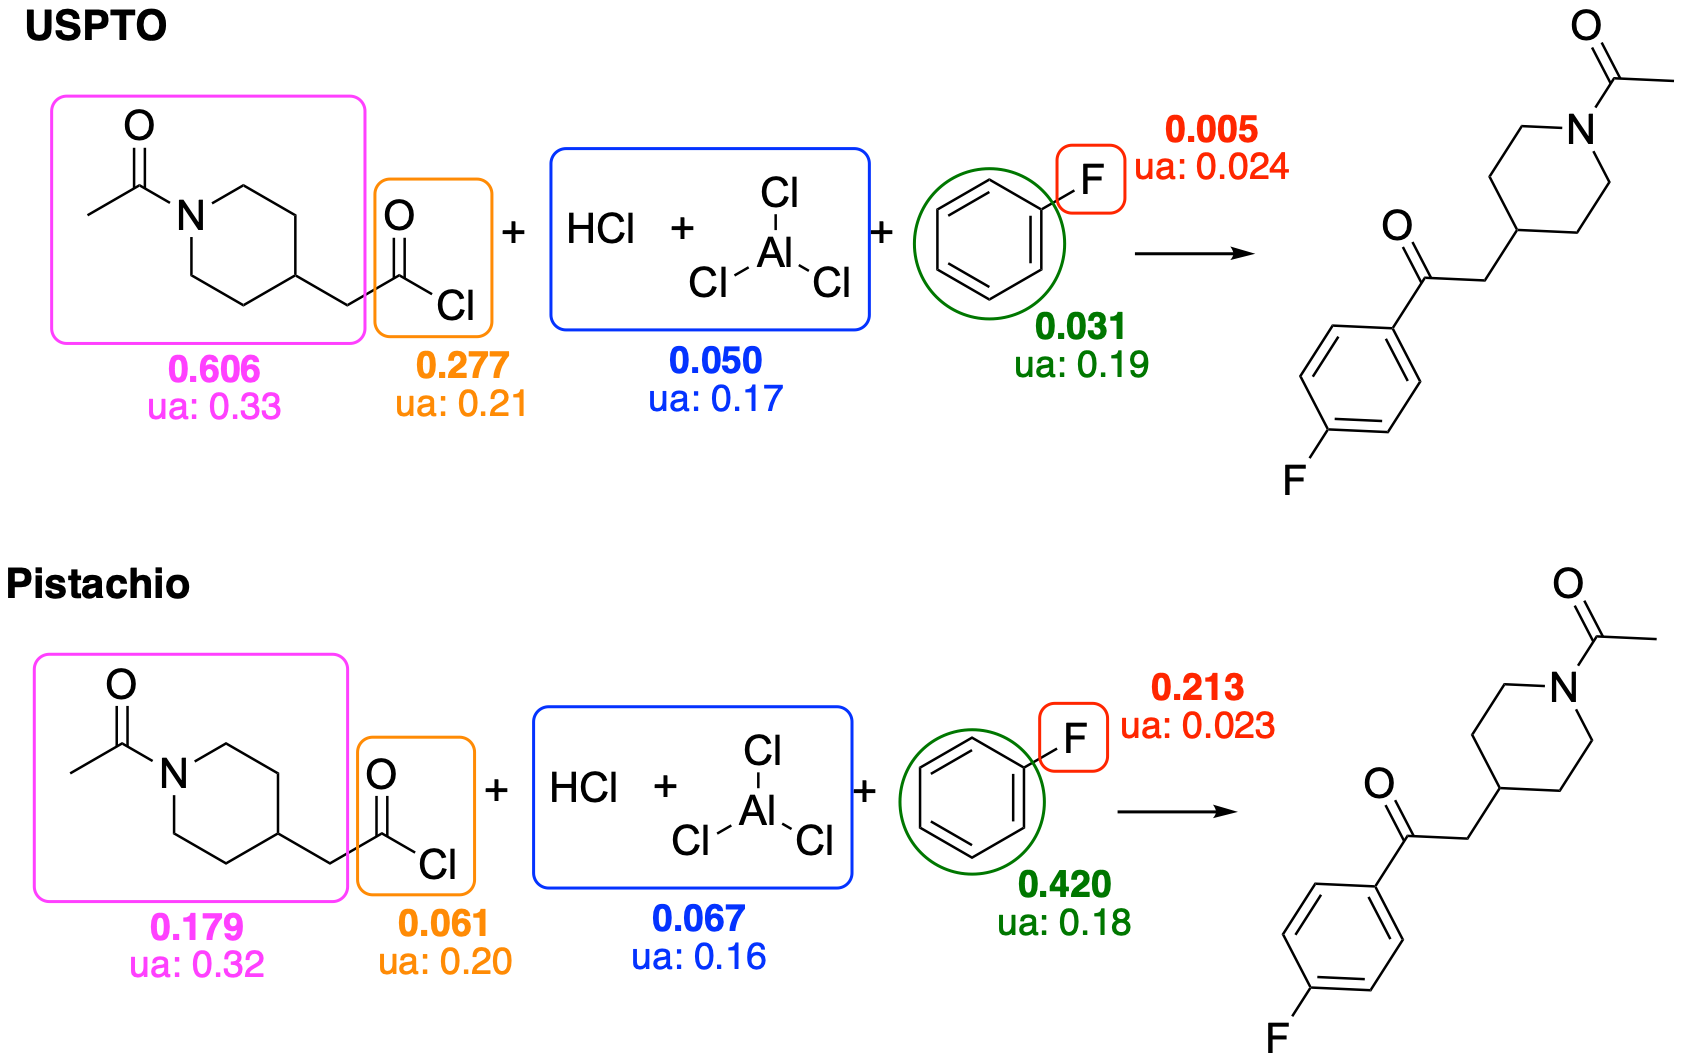
\includegraphics[width=0.8\textwidth]{Chapters/Transformer/Figs/sear_pred.png}
% % \caption[FC IG]{Both models predict the correct Friedel-Crafts acylation product but only the Pistachio model recognizes the importance of the -F atom in determining selectivity. The Integrated Gradients attributions are also shown along with the uniform attribution (ua) values. }
% % \label{fig:sear_pred}
% % \end{figure}

% % The predictions of the two models are shown in Fig~\ref{fig:sear_pred}. Both models predict the para selectivity correctly with confidence scores close to 1.0. When inspecting the IG attributions it can be seen that the USPTO model puts a very small weight on the Fluorine, only a fifth of the uniform attribution value. There is a large attribution given to the reagent though which does not affect the selectivity of this reaction at all. The attributions indicate that the USPTO transformer has not learnt the importance of F as the cause of para selectivity in these reactions. On the other hand the Pistachio transformer assigns a very high attribution value to F, suggesting that it has recognized the reason for the selectivity. 

% % Guided by the attributions we designed a number of adversarial examples where we have changed only the Fluorine part of the reactant-reagent input. This choice was motivated by the fact that according to the USPTO model the selectivity was driven by the reagents instead of the substituent on the benzene ring. If our interpretation is correct the model should keep predicting the para product even if a meta directing substituent is attached to the ring. The predictions of the models and the IG attributions of the meta directing groups are shown in Fig~\ref{fig:sear_adv}.

% % \begin{figure}[htbp!] 
% % \centering    
% % 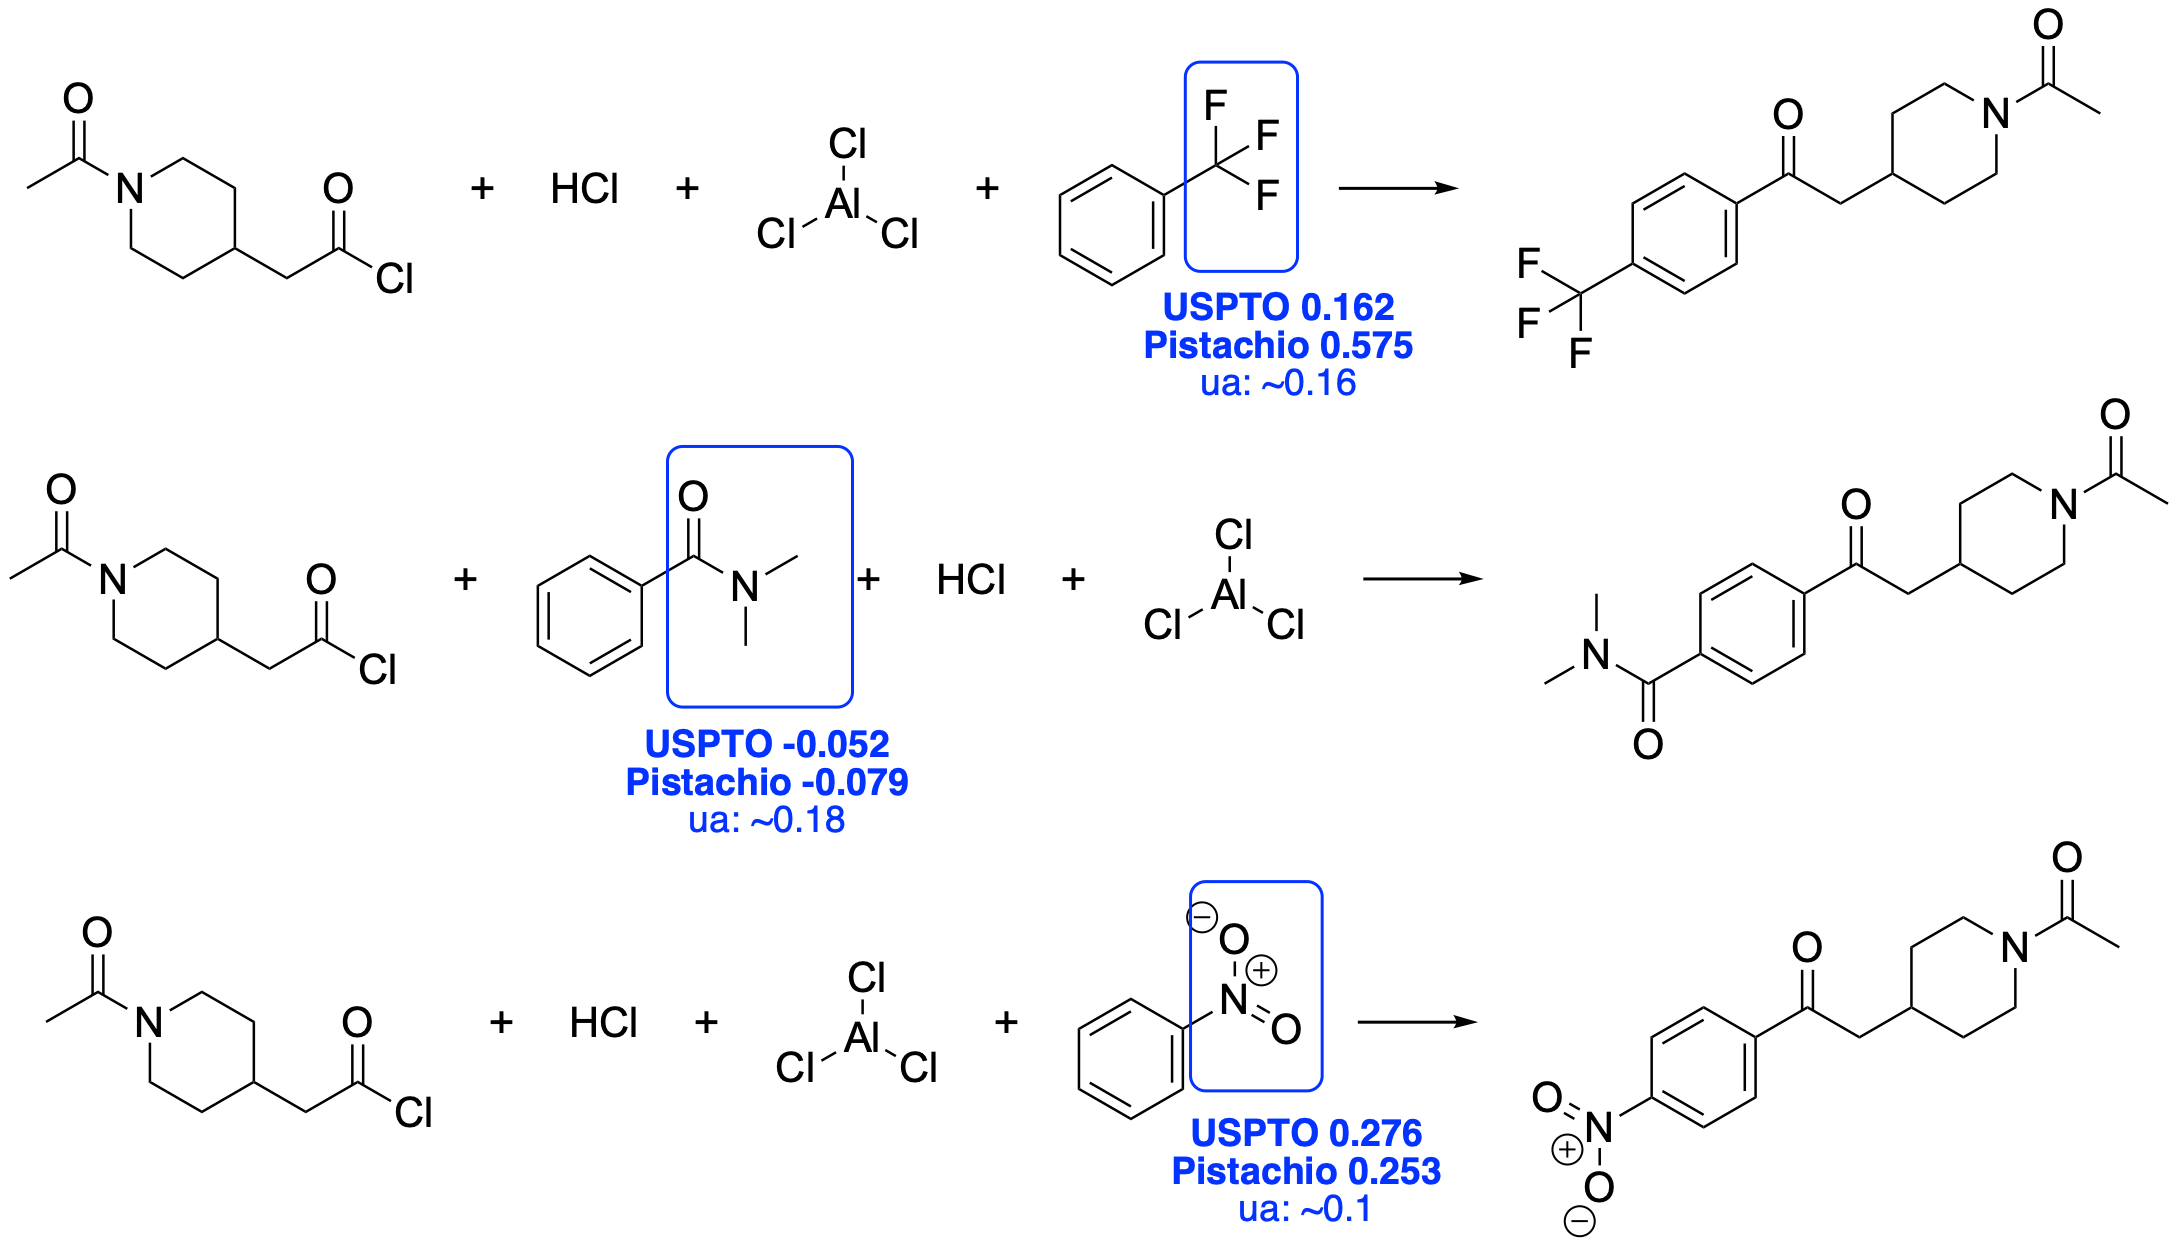
\includegraphics[width=1.0\textwidth]{Chapters/Transformer/Figs/sear_adv.png}
% % \caption[FC IG]{Adversarial examples designed using Fig~\ref{fig:sear_pred} reveal that both models can easily fail to predict the correct meta product. The uniform attribution (ua) values for the IGs are also shown. }
% % \label{fig:sear_adv}
% % \end{figure}

% % It can be seen that both transformer models fail in terms of predicting the meta directing effect of the substituents on the rings. In this case negative attributions favour the meta and positive the para product. There seems to be no correlation between the attribution values and the directing effect of the substituents, and even the Pistachio transformer is struggling with identifying the chemically important parts of the input. 

% % A suggestive observation is that in the second example the attributions on the meta directing group are negative, meaning that according to the models the amide group (correctly) favours the formation of the meta product. This agrees with chemical principles, but the model is still predicting the para to be the major product. We hypothesized that this might be due to biases in the training data, because if there are many more para substitution reactions than meta, the model could become biased towards predicting para substitutions even in the presence of meta directing groups. 

% % \begin{figure}[htbp!] 
% % \centering    
% % 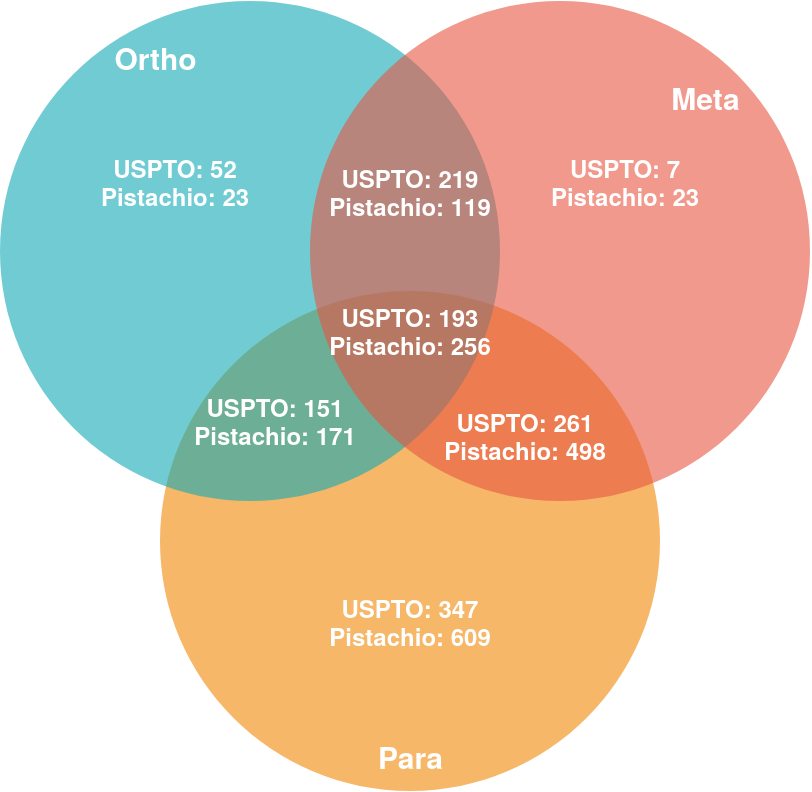
\includegraphics[width=0.65\textwidth]{Chapters/Transformer/Figs/sear_directing.png}
% % \caption[FC IG]{Counting the number Friedel-Crafts acylation reactions in the training sets with ortho, meta and para selectivities reveals an alarming bias -- the number of para reactions far outweigh those of meta or ortho reactions.}
% % \label{fig:sear_dir}
% % \end{figure}

% % To check if this hypothesis was correct we counted the number of ortho, meta and para Friedel-Crafts acylations in the training dataset using reaction templates. There was a large number of reactions matching multiple templates because often the benzene rings had multiple substituents on them. The results are summarized on Fig~\ref{fig:sear_dir}. 

% % The overall number of meta substitutions was 680 and 896 for the USPTO and Pistachio datasets respectively compared to the 952 and 1534 para substitutions. However, these numbers do not reveal the true extent of the bias as in our test case the benzene ring was only singly substituted. The number of reactions where there is only a single meta directing group on the ring is only 7 and 23 for the two datasets, which are extremely small numbers compared to those for a single para directing substituent which are 347 and 609, a ratio of 25-50 times.

% % This may result in the models not being able to learn meta directing substitution reactions because it can already achieve very high (~98\%) accuracy on the training set by always predicting the para product. The inclusion of further meta substitution reactions could considerably increase the models performance in real tasks. To confirm that the model would be able to learn the selectivities if the dataset was not biased, we probe the model with a synthetic dataset of para and meta Friedel-Crafts reactions in Sec.~\ref{subsec:synth_data}.

% % \subsection{Selective reduction of aldehydes and ketones}
% % Reduction of esters and aldehydes follow very well defined selectivity that is determined by the reducing agent. It is possible to reduce selectively an aldehyde or a ketone to alcohol in the presence of an ester. In this example the reduction of aldehydes using sodium-borohydride is examined \cite{Clayden2012}. If the Na is replaced by Li the reduction stops being selective to aldehydes and esters get reduced as well. The question is whether the models were able to learn the role of the cations in driving this subtle selectivity. An example reaction containing this selectivity is shown in Fig~\ref{fig:redu}.

% % \begin{figure}[htbp!] 
% % \centering    
% % 
\includegraphics[width=0.9\textwidth]{Chapters/Transformer/Figs/reduction.png}
% % \caption{An example of a reaction showing how NaBH\textsubscript{4} reduces the aldehydes selectively in the presence of an ester.}
% % \label{fig:redu}
% % \end{figure}

% % Both models are able to predict the product correctly with very high confidence (score > 0.95). In this case it is not immediately obvious what an interpretable attribution would be. One could argue that the selectivity is caused by Na\textsuperscript{+} because if we swap it to Li\textsuperscript{+} the other product would become the true product. The IG attributions on the \texttt{[Na+]} token are 0.013 and 0.017 for the USPTO and Pistachio models respectively, less than what the uniform attribution would be. This suggests that the models have not identified the importance of Na\textsuperscript{+} ion. 

% % To better understand the reliability of the predictions we attribute the reaction to the training data. For both models the most similar reactions (Fig~\ref{fig:redu_dat}) are BH\textsubscript{4} reductions of molecules containing both a ketone and an ester group. These examples suggest that both models have learnt this selectivity correctly, but they are not helping in understanding the role of the Na\textsuperscript{+}ion in the reaction.

% % \begin{figure}[htbp!] 
% % \centering    
% % 
\includegraphics[width=0.9\textwidth]{Chapters/Transformer/Figs/reduction_dat.png}
% % \caption{Data attribution to the reaction in Fig~\ref{fig:redu} suggests that both models have correctly learnt the selectivity of reduction.}
% % \label{fig:redu_dat}
% % \end{figure}

% % To investigate further if the models have learnt the importance of the cation in these reactions we designed an adversarial example where the only difference from the reaction on Fig~\ref{fig:redu} was the replacement of Na\textsuperscript{+} with Li\textsuperscript{+}. From Fig~\ref{fig:redu_adv} we see that the USPTO transformer keeps predicting the aldehyde being selectively reduced whereas the Pistachio model recognizes the change and predicts the correct product with both groups reduced. 

% % \begin{figure}[htbp!] 
% % \centering    
% % 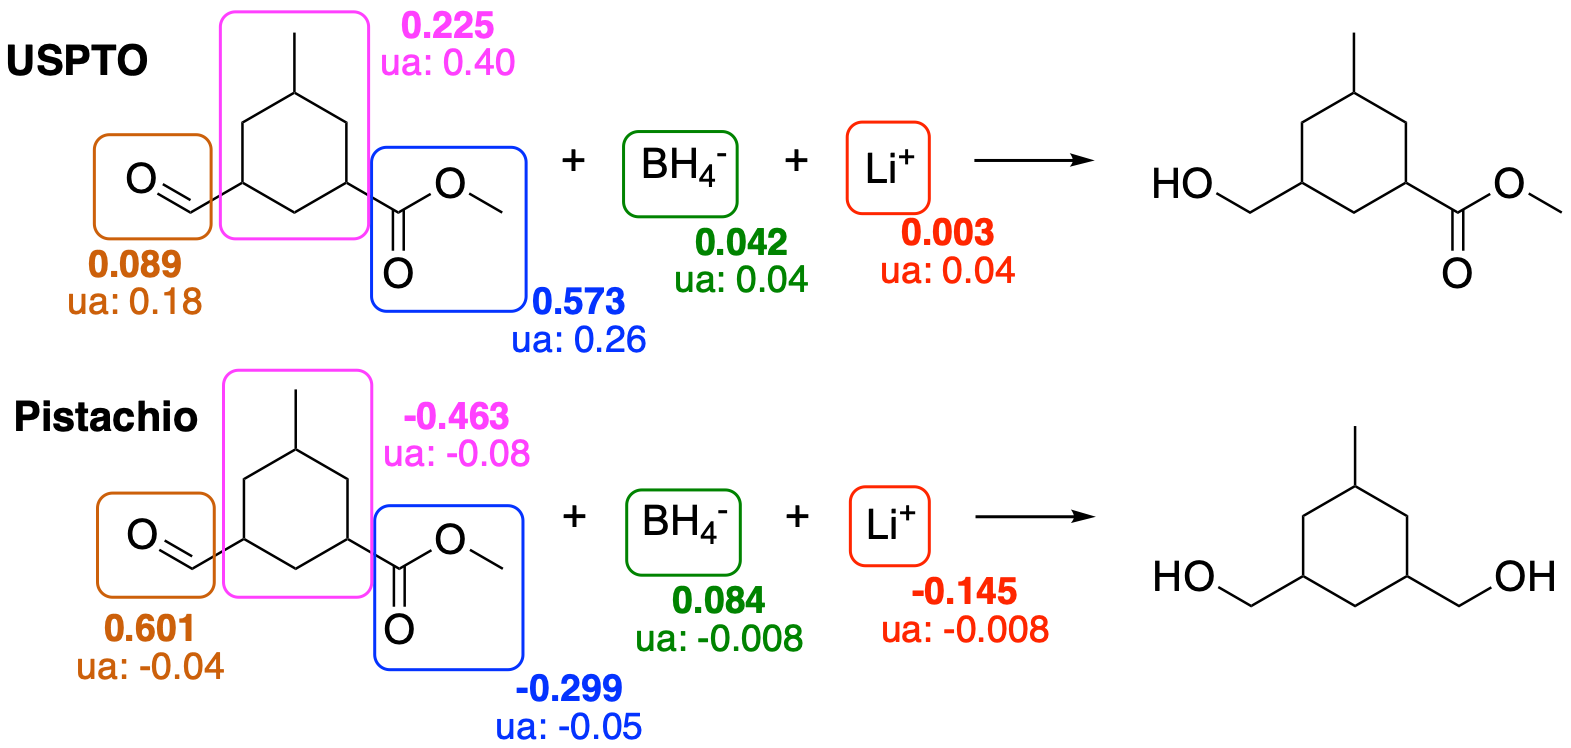
\includegraphics[width=0.9\textwidth]{Chapters/Transformer/Figs/redu_adv.png}
% % \caption{Adversarial example for the borohydride reduction in Fig~\ref{fig:redu} where the Na\textsuperscript{+} ion was replaced by Li\textsuperscript{+} ion. The USPTO model continues predicting the selective reduction of the aldehyde wrongly whereas the Pistachio model predicts the correct product -- the understanding of the models is reflecting in the IG attribution on the Li\textsuperscript{+} ion.}
% % \label{fig:redu_adv}
% % \end{figure}

% % To prove that one model was able to identify the importance of the cation and the other was not the IG attributions were generated and are shown in Fig~\ref{fig:redu_adv}. Here positive attributions favour the selective reduction, and the negative attributions favour the correct product. It is immediately obvious from the attributions that the USPTO model did not take into account the Li\textsuperscript{+} ion as it was given an attribution score that is an order of magnitude smaller than the uniform attribution value.

% % For the Pistachio model the probability score difference between the products was -0.21 and there was a lot of variation in attribution across different parts of the structure. The \texttt{[Li+]} token was given a very large negative attribution meaning that the model was strongly relying on it when making the correct prediction. Overall comparing the attributions it can be concluded that the USPTO model did not learn the chemistry of LiBH\textsubscript{4}, but the Pistachio one did. This can be due to the fact that the Pistachio model has seen more than 6 times more examples with this reagent. 

% % \subsection{Exploring the model with artificial data}
% % \label{subsec:synth_data}
% % One of the limitations of learning chemistry from patented and published reactions is that these reactions were designed by trained chemists who avoid transformations that have non-obvious selectivities. This makes it difficult for the models to infer the order of reactivity of functional groups. A further point is the effect of bias in the datasets on the models performance. To better understand these effect with full control over the experimental parameters, we have designed two artificial tasks where the training reaction data is generated using explicit SMARTS templates. 

% % In the first experiment we test whether the transformer model is able to learn selective chemistry if given enough data. We assembled a synthetic dataset of 90 000 reduction reactions. Carbon scaffolds were randomly selected from the ZINC database of drug-like molecules \cite{Irwin2005ZINCScreening}. To each scaffold we added an aldehyde group, an ester group, or both. Finally the 90 000 reactions, summarized in Table~\ref{table:red_datasets}, were obtained by applying one of three reduction templates shown in Fig~\ref{fig:redu_templates} to them. 

% % \begin{figure}[htbp!] 
% % \centering    
% % 
\includegraphics[width=0.6\textwidth]{Chapters/Transformer/Figs/redu_templates.png}
% % \caption[epoxide IG]{Three uniquely selective reduction templates are chosen to challenge the transformer's ability to learn selectivities if given enough data.}
% % \label{fig:redu_templates}
% % \end{figure}

% % \begin{table}[!h]
% % \caption{Number of reactions in the synthetic reduction datasets}
% % \centering
% % \label{table:red_datasets}
% % \begin{tabular}{m{0.17\textwidth}>{\centering}m{0.1\textwidth}>{\centering \arraybackslash}m{0.1\textwidth}>{\centering \arraybackslash}m{0.1\textwidth}}
% % \toprule
% %  \textbf{Subset} & \textbf{Aldehyde} & \textbf{Ester} & \textbf{Both}\\ 
% % \midrule
% % NaBH\textsubscript{4} & 20 000 & 0 & 10 000  \\
% % DIBAL & 0 & 20 000 & 10 000  \\
% % LiAlH\textsubscript{4} & 10 000 & 10 000 & 10 000  \\
% % \bottomrule
% % \end{tabular}
% % \end{table}

% % When training the transformer on this dataset we found that the only limiting factor in the performance of the model was its ability to reconstruct the sometimes tricky backbones of the molecules from the ZINC dataset. The selective chemistry was learnt (99\% top-1 accuracy) by the model in less than 10 000 steps. This shows that given sufficient data the model is able to learn selective transformations. To investigate how these findings are reflected in the IG attributions and verify that they are able to capture these empirical observations we generated the attributions for the reaction shown in Fig~\ref{fig:toy_attr}.

% % \begin{figure}[htbp!] 
% % \centering    
% % 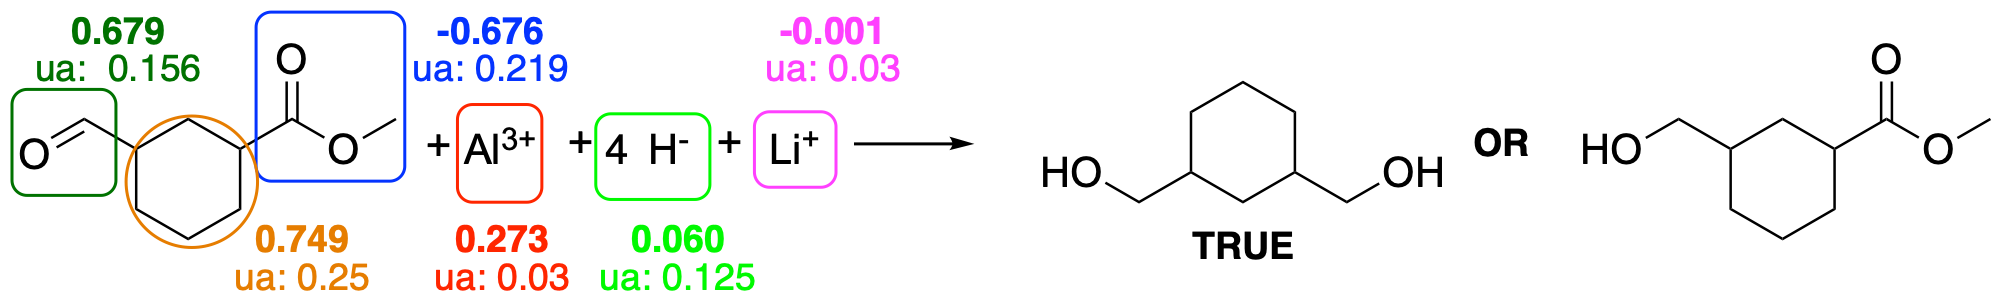
\includegraphics[width=1.00\textwidth]{Chapters/Transformer/Figs/toy_attr.png}
% % \caption{The model trained on artificial reduction data correctly attributes importance to the Al\textsuperscript{3+} ion.}
% % \label{fig:toy_attr}
% % \end{figure}

% % From the attributions we see that the model rightly gives high attribution to the Al\textsuperscript{3+} ion and small attribution to Li\textsuperscript{+}. This suggests that the model has learnt that it should only attend to one of the two tokens because they always appear together in the reactions. The H\textsuperscript{-} ions get a low attribution as expected. The attributions also verify that the model is finding the backbone part of the input very important, as reconstruction of the backbone is the most challenging aspect of making a correct prediction for this dataset of diverse backbones but restricted chemistry.

% % In the second more challenging synthetic experiment we investigated the models ability to learn the selectivity of aromatic electrophilic substitution reactions. By constructing balanced and biased datasets of Friedel-Crafts acylation reactions we hope to recover the observed behaviour in Sec.~\ref{subsec:friedel}. In the balanced and biased datasets we chose 10 para and 10 meta directing substituents which were placed on a benzene ring. For the last `super-biased' dataset, we only included three of the 10 meta directing substituents. These made the initial set of 20 reactant molecules which were reacted with a set of acyl chlorides generated by enumerating all possible straight carbon chains up to 8 carbons with a maximum of one double bond. This way we obtained 310 acyl chlorides that were reacted with the substituted benzenes to yield the meta or the para product. We use small carbon chains rather than the ZINC scaffolds to facilitate the learning of the backbones compared to learning the chemistry, which is partly why the dataset size was reduced as well and SMILES augmentation was applied. A summary of the training sets is shown in Table~\ref{table:synth_datasets}.

% % \begin{table}[!h]
% % \caption{Number of reactions in the synthetic Friedel-Crafts training datasets}
% % \centering
% % \label{table:synth_datasets}
% % \begin{tabular}{m{0.17\textwidth}>{\centering}m{0.1\textwidth}>{\centering \arraybackslash}m{0.1\textwidth}}
% % \toprule
% %   & \textbf{Meta} & \textbf{Para} \\ 
% % \midrule
% % Balanced & 3100 & 3100  \\
% % Biased & 310 & 2790  \\
% % Super-Biased & 30 & 3000  \\
% % \bottomrule
% % \end{tabular}
% % \end{table}

% % The USPTO and Pistachio transformers were trained for $\sim$300 and $\sim$100 epochs respectively, so this is the regime we wanted to investigate. We trained 10 transformer models on each of the datasets and saved checkpoints regularly. We created a test set using three meta directing and three para directing substituted benzenes combined with acyl chlorides not in the training sets, resulting in a balanced test set made up of 177 meta and 177 para substitution reactions. Using SMARTS template matching, we tested what proportion of the model predictions (with valid SMILES) are meta and para as a function of the number of epochs for different dataset biases. The results are shown in Fig~\ref{fig:synth_conv}. 

% % \begin{figure}[htbp!] 
% % \centering    
% % 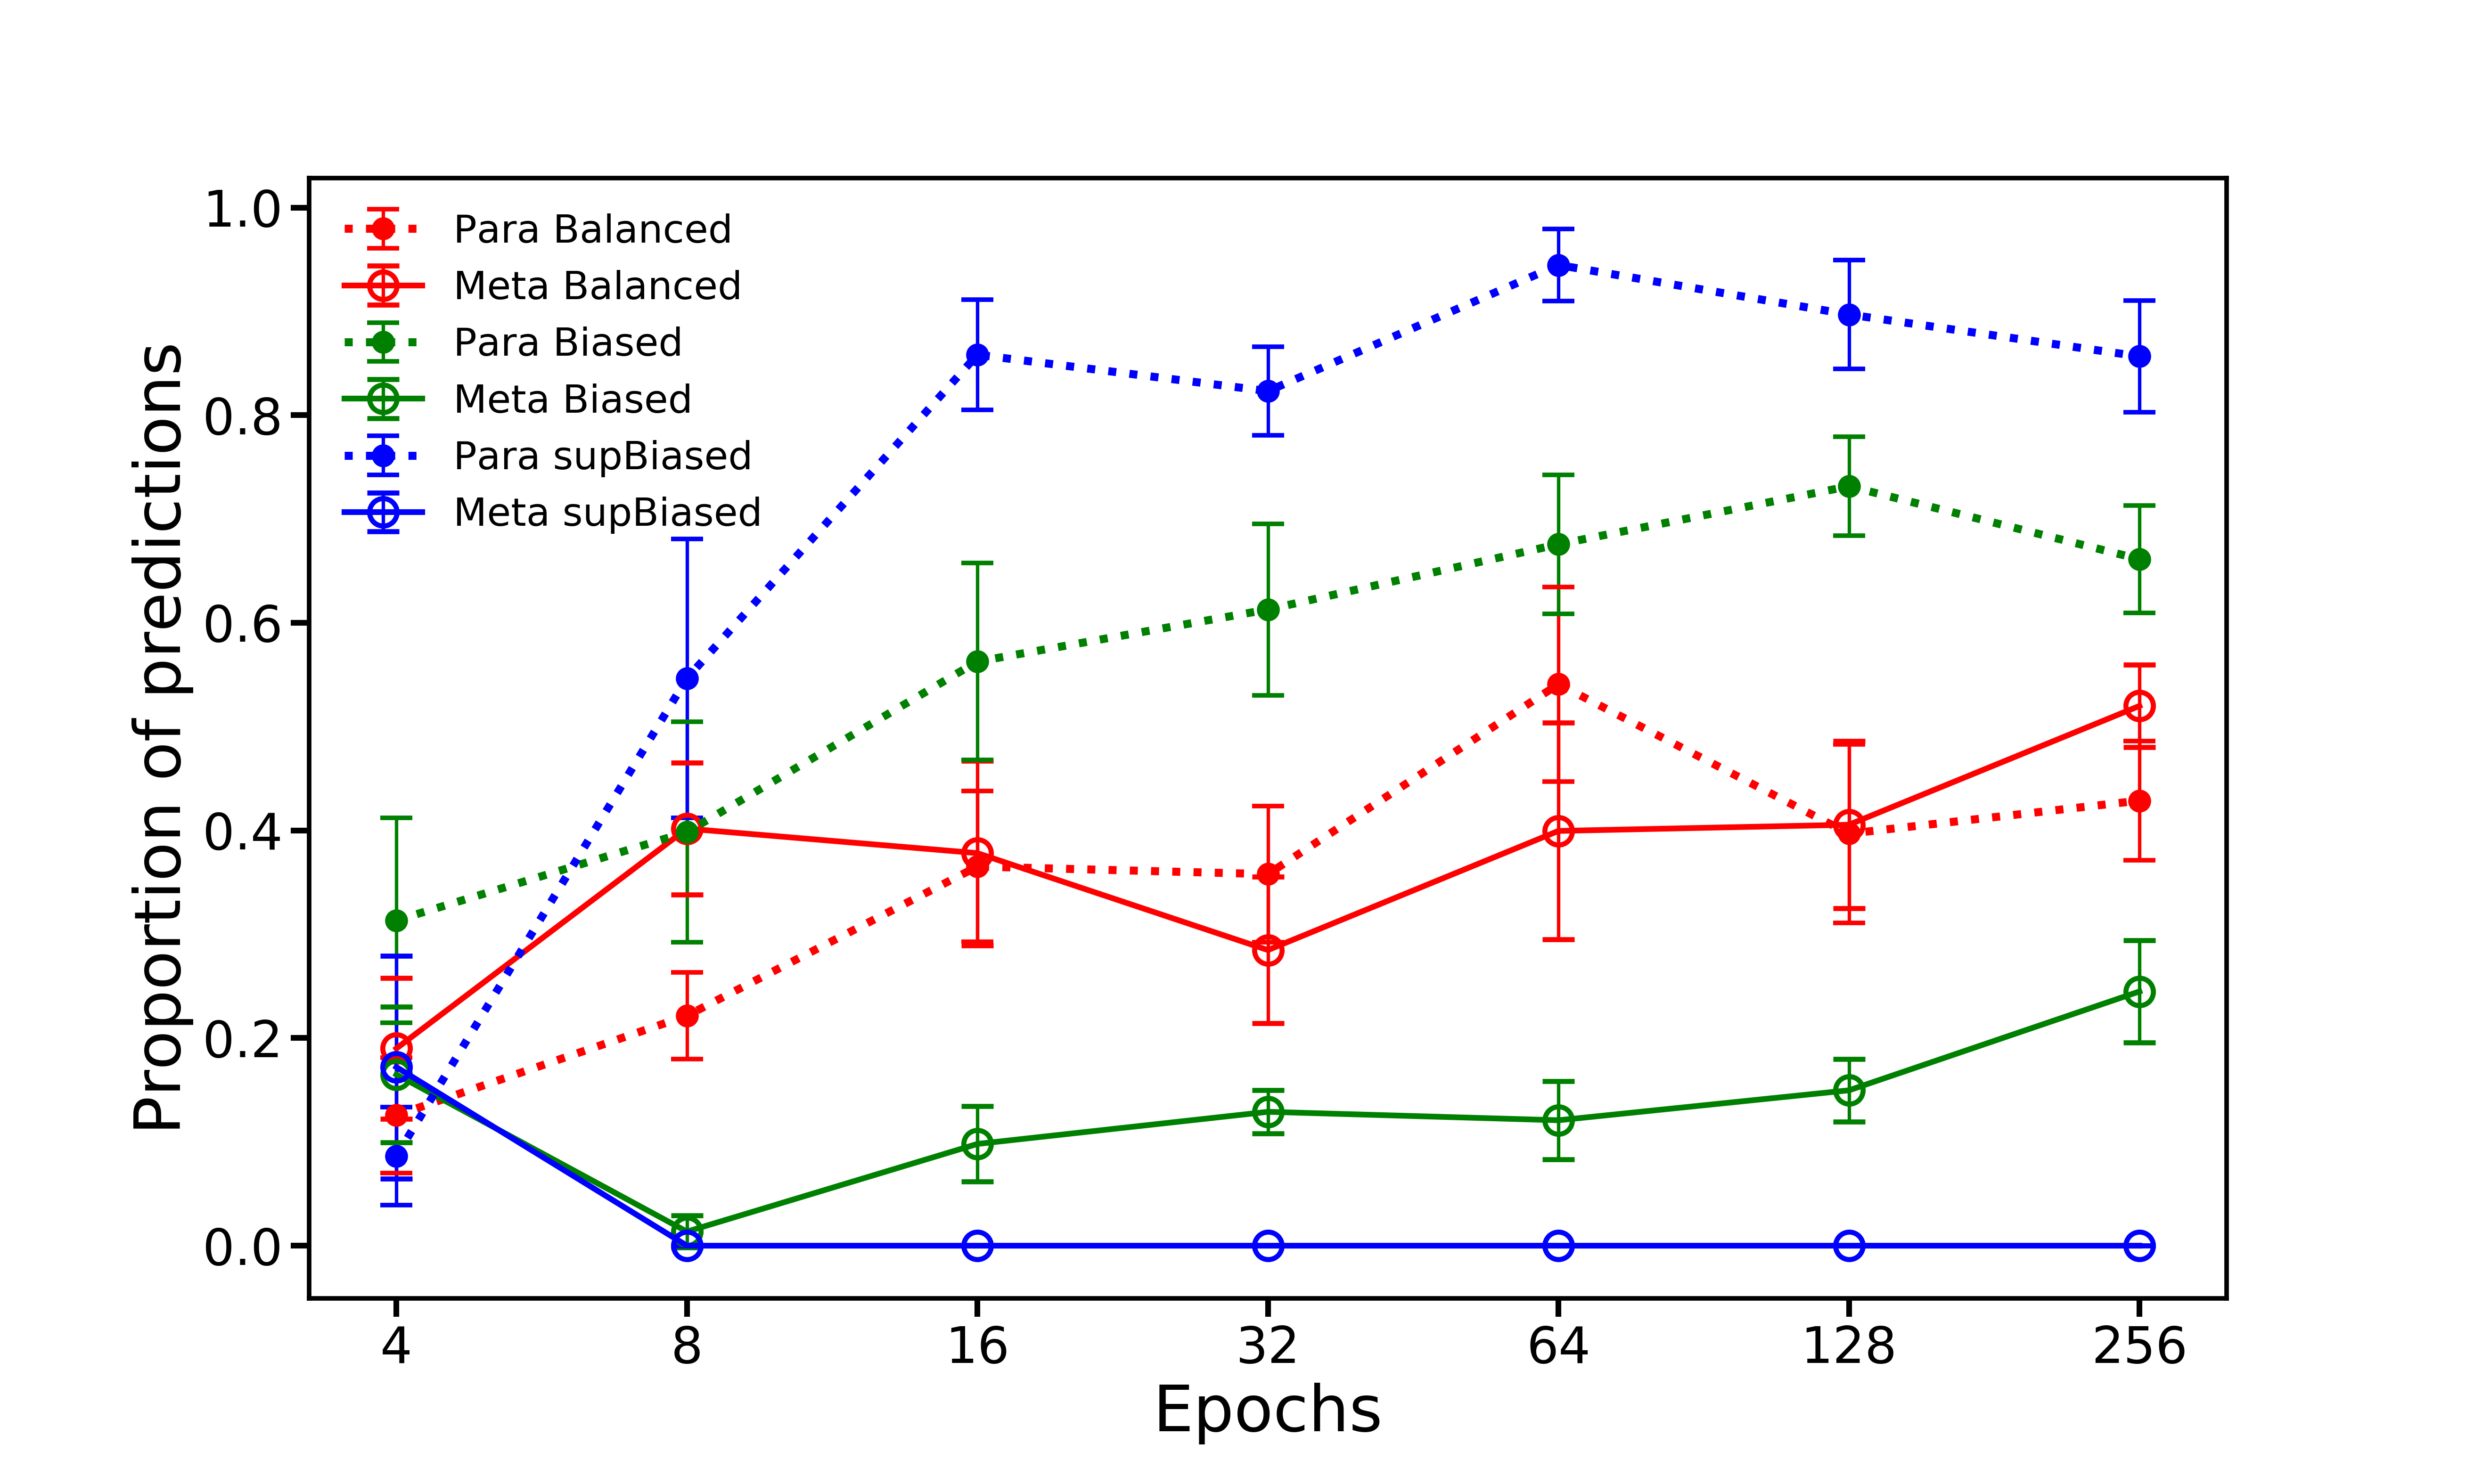
\includegraphics[width=1.0\textwidth]{Chapters/Transformer/Figs/synth_conv.png}
% % \caption{Dataset bias is reflected in the model predictions. The figure shows the proportion of para (solid line) and meta (dashed line) predictions on a balanced test set as a function of the number of training epochs for different biased training sets. }
% % \label{fig:synth_conv}
% % \end{figure}

% % We see that the balanced dataset converges quickly close to the correct ratio of 1:1 between meta and para predictions. On the other hand the bias in the training set is reflected in the predictions of the other two models, in the case of the super-biased model to the extent that it does not predict any meta products. This is particularly revealing because that is the training set whose ratio is closest to that found in the USPTO and Pistachio datasets. This serves as empirical proof that the observed failure to predict the meta substituent in Sec.~\ref{subsec:friedel} is the result of biases in the dataset. 

% % Finally we ran the models to convergence to see if eventually they are able to predict the correct structures. After $\sim$4 000 epochs the ratio of meta to para was exactly 1:1 for the balanced dataset and about 3:5 on both the biased and super-biased datasets. This shows that by training longer the effect of dataset bias can be mitigated, but it cannot be removed altogether. 

% % \subsection{Outlook}
% % \label{chap:conclusion}

% % Chemical reaction prediction models have undergone a revolution driven by innovations in the field of machine learning. This large increase in accuracy came at the expense of interpretability as expert crafted rules and reaction mechanisms gave way to black-box deep learning models. 

% % The predictions of machine learning models depend on two essential components. One of them is the training data which acts as an upper limit to the performance of the model. Any machine learning model can be only as good as the data it was trained on. The other ingredient is the input that is processed and turned into the prediction. We have developed two robust methods for interpreting and testing reaction prediction models focusing on each of these two ingredients, and applied them to analyse the Molecular Transformer which is the current state-of-the-art model. 

% % The first method builds on the Integrated Gradients method \cite{Sundararajan2017AxiomaticNetworks} for attributing the prediction of neural network models to parts of the input. This method has been used to identify which parts of the inputs to the model are important when predicting typical selective chemical reactions. It has been found that often the model does not identify chemically important substructures, demonstrated by the design of adversarial examples based on the attributions which fool the model.

% % The other method we developed attributes the predictions of the model to training data. We averaged the vector outputs from the last encoder layer of the Molecular Transformer to define a similarity metric between different reactions, as understood by the model. Attributing back to training data serves multiple purposes in the case of reaction prediction. It can either support or invalidate a prediction by telling the user which are the most similar training reactions according to the model. Furthermore this can be used to identify unknown trends or biases in the dataset or sometimes even to identify erroneous training examples. 

% % Using evidence from these attribution methods, we hypothesized that many of the erroneous predictions of the Molecular Transformer model stem from data biases. We have validated this hypothesis by designing an artificial dataset of Friedel-Crafts acylation reactions where we could show how biases in the dataset manifest in the predictions of the model. In addition, we observe that the model trained on the Pistachio dataset had in general better predictions and much better calibrated uncertainty scores, in spite of the fact that this model only achieved 76\% test-set accuracy. This suggests that Pistachio is not as biased as USPTO, and hints that the addition of training data can substantially improve model performance. 

% % From these results we believe that for reaction prediction, the Top-$N$ accuracy from testing on randomly chosen held-out test sets do not provide an adequate measure of the models true performance and generalization ability. We believe that this is partly results from the fact that publications and patents often contain reaction carried out on a series of analogous reactants. Therefore there is a high chance that essentially identical reactions end up in the training and test sets. A more honest measurement of the model's true generalizability could be realized by only including reactions in the test-set whose products have a low similarity to the products in the training set. The exploration of this idea is the subject of further work. 

% % Overall, from this work we believe that improvements to the training data can be just as impactful as improving the machine learning models themselves. By demonstrating the power of interpretability methods when rigorously applied to scientific questions, we have shown that these methods can be useful beyond just giving explanations of predictions by exposing dataset biases. Applying our approach for data and input interpretation beyond chemical reaction prediction to other fields will likely be equally constructive, illuminating the path to improved training data and hence improved artificial intelligence models.

